% =====================================================================
%  The Foreign Exchange Rate  --  merged chapter (all four members)
%  Introduction to Economics, Monsoon 2026
%  Build:  python source/build_book.py   then   latexmk main.tex  (XeLaTeX)
% =====================================================================
\documentclass[11pt]{article}
\usepackage{fxstyle}
\usepackage{xurl}

\begin{document}

\chaptertitle{Introduction to Economics \textperiodcentered{} Teaching chapter}
             {The Foreign Exchange Rate}
             {What is the rupee worth, and why does it keep changing?}

% ============================================================
%  INTRODUCTION: Meera's dollar problem        (Member 1)
%  Main-text words: see word count in README (boxes excluded)
% ============================================================
\section*{Introduction: Meera's dollar problem}
\addcontentsline{toc}{section}{Introduction}

In October 2026, Meera, a Class 12 student in Chennai, got the email her family had been waiting for: a college in the United States had offered her a place. The first-year fees were US\$40,000, exactly what the college had charged a year earlier. Yet when her father asked his bank what the fees would cost in rupees, the answer was about ₹2.5 lakh more than it would have been a year before.\sidenote{The fees are hypothetical. The exchange rates are real closing rates: ₹88.67 per US dollar on 13 October 2025 (Business Standard, 2025b) and ₹95.05 on 15 October 2026 (HDFC Sky, 2026). 40,000 × (95.05 − 88.67) = ₹2,55,200.} The college had not raised its price. The price of the dollar had gone up.

Meera's uncle Ravi, an electrician in Dubai, had the opposite surprise. Every month he sends part of his salary home to his parents in Thanjavur. This year the same amount arrived as more rupees than before.

One family, one price, and two very different outcomes. This chapter explains what that price is, who sets it, and why it keeps moving.

\begin{keypoints}{Questions this chapter answers}
\begin{itemize}
  \item Why does one country's money have a price in another country's money?
  \item Who buys and sells currencies, and why?
  \item What decides that price, and why does it change so often?
  \item How do countries, and the Reserve Bank of India, manage their exchange rates?
  \item Who gains and who loses when the rupee rises or falls?
\end{itemize}
\end{keypoints}
            % Member 1
% ============================================================
%  SECTION 1: What is an exchange rate?          (Member 1)
% ============================================================
\section{What is an exchange rate?}\label{sec:exrate}

Chai in Chennai is paid for in rupees, but coffee in New York needs US dollars and a meal in Dubai needs dirhams. So whenever goods, services or savings cross a border, one currency has to be swapped for another. The price of that swap is the \keyterm{exchange rate}{The price of one currency in terms of another, for example ₹95 per US dollar.}: the price of one currency in terms of another (National Council of Educational Research and Training [NCERT], 2007). In India it is set mainly by buyers and sellers in a market, and like the price of onions it can change from minute to minute.

Indian banks write the rate as a \keyterm{direct quote}{The price of one unit of foreign currency in home currency, e.g.\ US\$1 = ₹95.}, ``US\$1 = ₹95'', which is the number of rupees needed to buy one dollar (Jayadev, 2021). Flip it and you get the \keyterm{indirect quote}{How much foreign currency one unit of home currency buys, e.g.\ ₹1 = US\$0.0105.}, ``₹1 = US\$0.0105'', which is the number of dollars one rupee buys. This chapter always uses the direct quote, rupees per dollar (₹/\$), so a bigger number means a weaker rupee. At ₹95 instead of ₹88, every rupee buys fewer dollars \seesec{sec:appdep}.

\begin{figure}[htbp]
  \centering
  \begin{minipage}[c]{0.40\linewidth}
    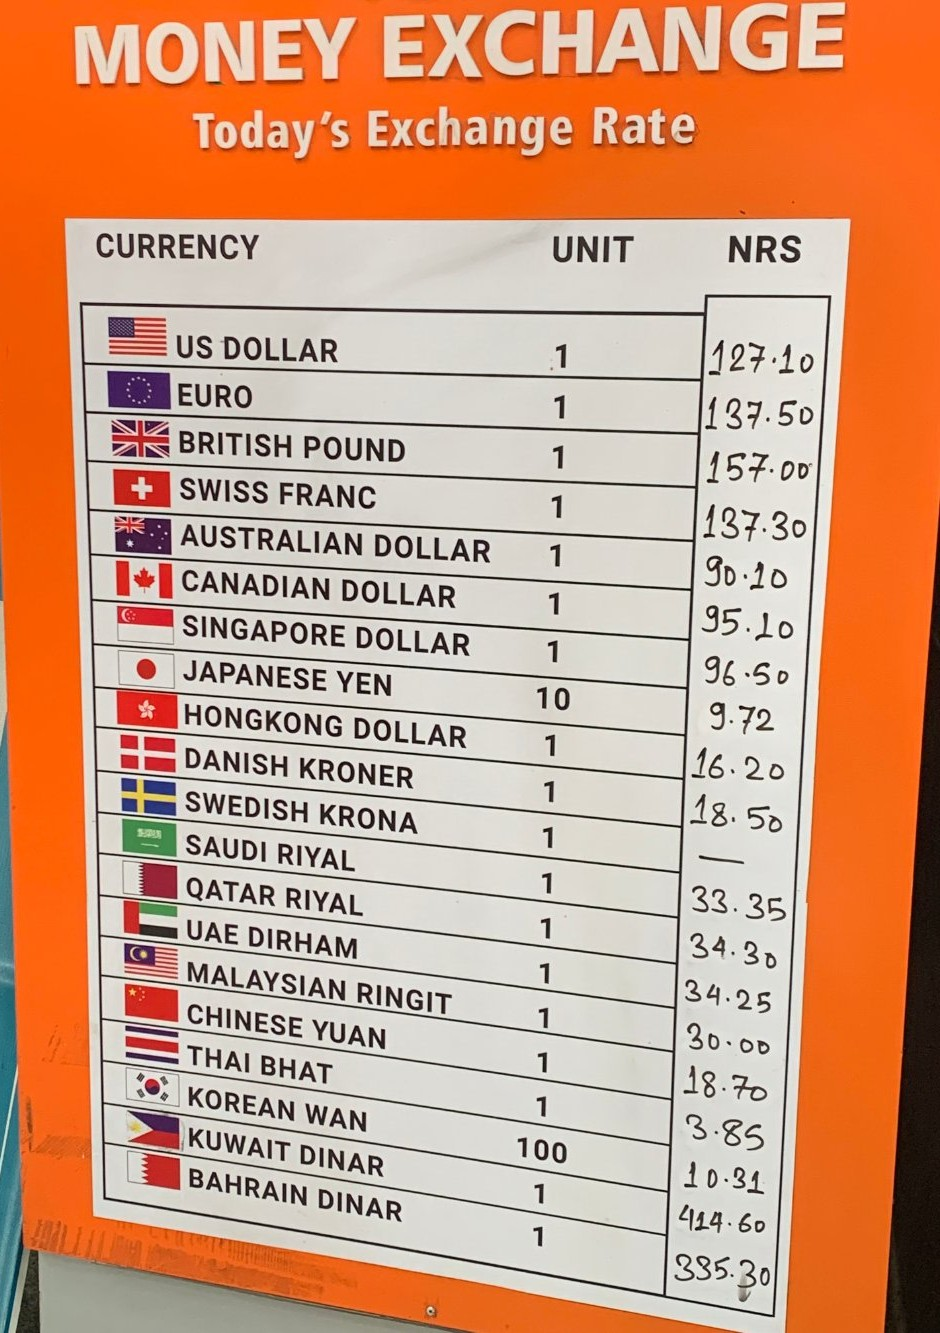
\includegraphics[width=\linewidth]{images/kathmandu_board.jpg}
  \end{minipage}\hfill
  \begin{minipage}[c]{0.56\linewidth}
    \caption{A money exchange board at Kathmandu airport, January 2023.}
    \label{fig:m1-board}
    \small\sffamily
    Each row is a \emph{direct quote}: the price of one unit of a foreign currency in Nepalese rupees (NRs). A US dollar costs NRs~127.10 and a UAE dirham, the currency Ravi earns, about NRs~34. The Japanese yen is priced per 10 yen, because a single yen is worth very little.
    \figsource{Photograph by Chainwit. (2023), \href{https://commons.wikimedia.org/wiki/File:Arrival_at_Kathmandu_Tribhuvan_Airport_(01-2023)_-_img_06.jpg}{Wikimedia Commons}, \href{https://creativecommons.org/licenses/by/4.0/}{CC BY 4.0}, cropped.}
  \end{minipage}
\end{figure}

\begin{didyouknow}{Every board hides two prices}
Banks and money changers quote two rates for each currency: a lower rate at which they buy it from you and a higher rate at which they sell it to you. Suppose a bank buys dollars at ₹93.50 and sells them at ₹96.50. Change ₹10,000 into dollars and you get US\$103.63. Change them straight back and you get only ₹9,689. The missing ₹311 is the bank's earning, called the \textbf{spread}. Spreads are usually widest for cash at airport counters, which is why travellers lose the most there.
\figsource{The rates in this example are hypothetical.}
\end{didyouknow}

\subsection{Why everyone watches the dollar}
Why does the news talk only about the rupee's price in dollars? Because the dollar is the world's working currency. In April 2025 it was on one side of 89 per cent of all currency trades (Bank for International Settlements [BIS], 2025). Crude oil, India's biggest import, is priced in dollars, and only about 6 per cent of India's exports are invoiced in rupees (Reserve Bank of India [RBI], 2026a). Since July 2022 the RBI has allowed Indian firms to settle foreign trade in rupees (RBI, 2022), but most still choose the dollar, because almost everyone, everywhere, will accept it.

The dollar even reaches currencies that seem unrelated. The UAE dirham, which Ravi earns, has been fixed at 3.6725 dirhams per US dollar since 1997 (Nagraj, 2024). So when a dollar costs more rupees, so does a dirham, and every dirham Ravi sends home turns into more rupees.
    % Member 1
% ============================================================
%  SECTION 2: The foreign exchange market        (Member 1)
% ============================================================
\section{The foreign exchange market: who needs dollars and who supplies them?}\label{sec:forex}

Currencies are bought and sold in the \keyterm{foreign exchange market}{The market in which currencies are traded for one another. Also called the forex market.}, or forex market. It has no building and no closing bell. It is a worldwide network of banks, dealers and large firms that trade with each other electronically, and as the day moves from Tokyo and Singapore to Mumbai, London and New York, the trading moves with it (Greenlaw et al., 2022).

Figure~\ref{fig:m1-flow} sorts the people in this market into two groups. Importers, students and travellers abroad, Indians investing abroad and anyone repaying a foreign loan need dollars. Together they make up the \keyterm{demand for foreign exchange}{The foreign currency that residents want, to pay for imports, study and travel abroad, investment abroad and foreign loans.}. Exporters like Selvi, whose garment unit in Tiruppur sells T-shirts to American shops, workers abroad like Ravi who send home \keyterm{remittances}{Money that people working abroad send home to their families.}, foreign tourists and foreign investors all bring dollars in. They make up the \keyterm{supply of foreign exchange}{The foreign currency flowing into a country from its exports, remittances, tourists and foreign investment.} (NCERT, 2007). Every deal is two purchases at once: when Meera's father buys dollars, he is also selling rupees (Greenlaw et al., 2022). The exchange rate is the price at which the two sides match \seesec{sec:ds}.

\begin{figure}[!htb]
  \centering
  \resizebox{\linewidth}{!}{% Figure M1-2: who demands and who supplies US dollars in India's forex market.
% Drawn in TikZ so it stays sharp and editable. Uses colours from fxstyle.sty.
\begin{tikzpicture}[
  font=\sffamily\small, every node/.append style={execute at begin node={\spaceskip=0.24em plus 0.04em minus 0.02em\relax}},
  item/.style={draw=none, fill=white, rounded corners=1.2mm, minimum height=9.2mm,
               text width=48mm, align=left, execute at begin node={\hyphenpenalty=10000\relax}, inner xsep=7pt, inner ysep=3pt},
  head/.style={text=white, font=\sffamily\bfseries, align=center, text width=52mm,
               minimum height=12mm, rounded corners=1.5mm},
  who/.style={font=\sffamily\scriptsize\itshape, text=fxmuted},
  flow/.style={-{Stealth[length=3.2mm,width=2.6mm]}, line width=1.6pt},
]
% ---- left column: demand ----
\node[head, fill=fxorange] (dh) at (0,0)
  {Who wants dollars?\\[-1pt]{\footnotesize\mdseries demand for foreign exchange}};
\node[item, below=3mm of dh] (d1) {\textbf{Importers}\\[-1pt]{\footnotesize crude oil, gold, electronics, machines}};
\node[item, below=2mm of d1] (d2) {\textbf{Students and travellers abroad}\\[-1pt]{\footnotesize \textcolor{fxorange}{e.g.\ Meera's college fees}}};
\node[item, below=2mm of d2] (d3) {\textbf{Indians investing abroad}\\[-1pt]{\footnotesize shares, property, firms}};
\node[item, below=2mm of d3] (d4) {\textbf{Repaying foreign loans}\\[-1pt]{\footnotesize firms and government}};
\begin{scope}[on background layer]
  \node[fill=fxorange!10, rounded corners=2mm, inner sep=3mm, fit=(dh)(d4)] (dbox) {};
\end{scope}

% ---- right column: supply ----
\node[head, fill=fxteal] (sh) at (13.4,0)
  {Who brings dollars in?\\[-1pt]{\footnotesize\mdseries supply of foreign exchange}};
\node[item, below=3mm of sh] (s1) {\textbf{Exporters}\\[-1pt]{\footnotesize \textcolor{fxteal}{e.g.\ Selvi's T-shirts}, IT services}};
\node[item, below=2mm of s1] (s2) {\textbf{Remittances}\\[-1pt]{\footnotesize \textcolor{fxteal}{e.g.\ Ravi's money from Dubai}}};
\node[item, below=2mm of s2] (s3) {\textbf{Foreign tourists in India}\\[-1pt]{\footnotesize hotels, travel, shopping}};
\node[item, below=2mm of s3] (s4) {\textbf{Foreigners investing in India}\\[-1pt]{\footnotesize FDI and FPI}};
\begin{scope}[on background layer]
  \node[fill=fxteal!10, rounded corners=2mm, inner sep=3mm, fit=(sh)(s4)] (sbox) {};
\end{scope}

% ---- centre: the market ----
\coordinate (mid) at ($(dbox.east)!0.5!(sbox.west)$);
\node[fill=fxnavy, text=white, rounded corners=3mm, text width=36mm, align=center,
      minimum height=34mm, inner sep=6pt] (mkt) at (mid)
  {\heavysans\large Foreign\\exchange market\\[5pt]
   {\footnotesize\sffamily banks and other authorised dealers, regulated by the RBI}};
\node[fill=white, draw=fxnavy, line width=0.8pt, rounded corners=1.5mm, below=4mm of mkt,
      align=center, text width=34mm, inner sep=4pt] (price)
  {{\footnotesize\color{fxmuted}the price that clears it}\\[-1pt]{\heavysans\color{fxnavy}\large ₹ per US dollar}};

% ---- flows ----
\draw[flow, fxorange] (dbox.east |- mkt.150) -- (mkt.150)
  node[pos=0.5, above=1pt, font=\sffamily\scriptsize\bfseries, text=fxorange, align=center] {offer rupees,\\ want dollars};
\draw[flow, fxteal] (sbox.west |- mkt.30) -- (mkt.30)
  node[pos=0.5, above=1pt, font=\sffamily\scriptsize\bfseries, text=fxteal, align=center] {offer dollars,\\ want rupees};
\end{tikzpicture}
}
  \caption{Who wants dollars and who brings them in.}
  \label{fig:m1-flow}
  {\raggedright\small\sffamily Each group on the left offers rupees to get dollars. Each group on the right offers dollars to get rupees.\par}
  \figsource{Drawn by the authors, based on NCERT (2007, Chapter 6) and Greenlaw et al. (2022, Section 29.1).}
\end{figure}

\subsection{Most currency trading is not about trade}
In April 2025, about US\$9.6 trillion worth of currencies changed hands every day (BIS, 2025). All the world's exports of goods and services in 2024 were worth about 33 trillion dollars (United Nations Conference on Trade and Development [UNCTAD], 2025). So the forex market trades a whole year of world exports in less than four days. Most of this trading is done by banks and investors moving savings between countries.

Investors come in two kinds. \keyterm{Foreign direct investment (FDI)}{Buying a lasting stake (10\% or more) in a business abroad, or setting one up.} buys a lasting stake in a business, like a carmaker building a factory near Chennai, and it stays for years. \keyterm{Foreign portfolio investment (FPI)}{Buying shares and bonds (holdings under 10\%), which can be sold quickly.} buys shares and bonds, and it can leave in a single day (Greenlaw et al., 2022). That is why its comings and goings can jolt the rupee \seesec{sec:moves}.

To buy dollars for the fees, Meera's father will simply walk into his bank in Chennai. Under the Foreign Exchange Management Act, 1999, only banks and firms licensed by the RBI, such as \keyterm{authorised dealers}{Banks and firms licensed by the RBI under FEMA, 1999, to buy and sell foreign currency.} and money changers, may deal in foreign currency. They trade with customers, with each other and with banks abroad, while the RBI makes the rules and, at times, buys or sells dollars itself \seesec{sec:reserves}.

\begin{casestudy}{Selvi's three-month gamble}
In October, Selvi agrees to sell T-shirts worth US\$20,000 to a shop in New York, which will pay in January. At today's rate of ₹95, that is ₹19 lakh. But if the rupee strengthens to ₹90 by January, she will receive only ₹18 lakh, and her profit could vanish. To avoid the gamble, Selvi can sign a \textbf{forward contract} with her bank today, fixing the rate at which the bank will buy her dollars in January. The rate for a deal settled today is the \textbf{spot rate}. A rate agreed today for a deal in the future is a \textbf{forward rate}. Importers use the same tool to protect themselves from a weaker rupee.
\figsource{The figures in this example are hypothetical.}
\end{casestudy}

\begin{economistsfacts}{Ravi is one of millions}
\centering
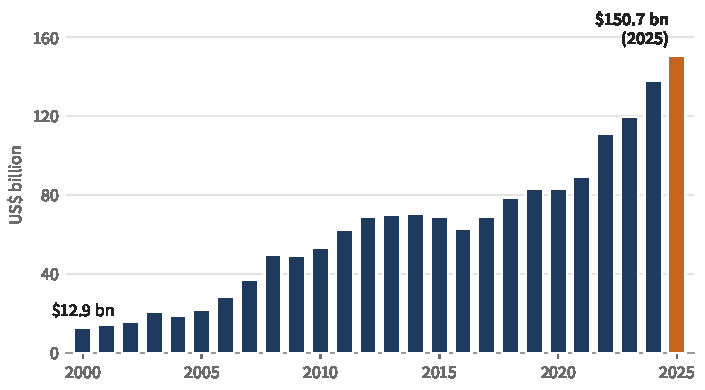
\includegraphics[width=\linewidth]{figures/remittances.pdf}
\captionof{figure}{Remittances received by India, 2000--2025 (US\$ billion).}\label{fig:m1-remit}
\figsource{World Bank (2026a), World Development Indicators, series BX.TRF.PWKR.CD.DT.}
\raggedright
In 2025, Indians working abroad sent home \textbf{US\$150.7 billion}, more than any other country received and more than twice as much as Mexico, the next-largest recipient (World Bank, 2026a). Where the money comes from is changing. In 2020-21 the US sent 23.4 per cent of it and the UAE 18.0 per cent. By 2023-24 the US share had risen to 27.7 per cent, while the UAE's had barely moved, to 19.2 per cent. An RBI study links this to more skilled Indians working in advanced economies (Gajbhiye et al., 2025).\par
\textbf{Read the chart.} (a) Roughly how many times larger were remittances in 2025 than in 2000? (b) In which year did they fall most sharply, and what might explain it?
\answers{(a) About 12 times (150.7 ÷ 12.9 ≈ 11.7). (b) 2016, when they fell about 9 per cent. The World Bank linked the fall to low oil prices and government spending cuts in the Gulf countries, where many Indians work (World Bank, 2017).}
\end{economistsfacts}

\begin{exercise}{Dollars in or dollars out?}
For each transaction, decide whether it adds to India's \emph{demand} for dollars or to the \emph{supply} of dollars.
\begin{enumerate}[label=(\alph*), leftmargin=2em]
  \item Meera's father pays her first-year fees.
  \item Ravi sends 3,000 dirhams to his parents in Thanjavur.
  \item A shop in New York pays Selvi for 5,000 T-shirts.
  \item A Japanese carmaker builds a new factory in Tamil Nadu.
  \item An Indian oil company buys a shipload of crude oil.
  \item An American investor sells her Indian shares and takes the money home.
  \item A family from Germany spends a week on a Kerala houseboat.
\end{enumerate}
\answers{Supply: (b), (c), (d), (g). Demand: (a), (e), (f).}
\end{exercise}
% [removed at merge] Member 1's "Watch and learn" box: the same Khan Academy
% video is listed first in Further learning at the end of the chapter.
     % Member 1
% ============================================================
%  SECTION 3 (was A): The rupee's account book   (Member 1)
%  Defines "current account deficit" used in Sections 9 and 11
% ============================================================
\section{The rupee's account book: the balance of payments}\label{sec:bop}

Every dollar that enters or leaves India is written down in the \keyterm{balance of payments (BoP)}{The record of all economic transactions between a country's residents and the rest of the world over a period.}, the record of all economic transactions between the residents of a country and the rest of the world over a period such as a year (NCERT, 2007). The \keyterm{current account}{The part of the BoP that records trade in goods and services, income and transfers.} records trade in goods and services, along with income and transfers such as remittances. The \keyterm{capital account}{The part of the BoP that records the buying and selling of assets, such as FDI, FPI and loans.} records the buying and selling of assets, such as FDI, FPI and foreign loans. When a country spends more foreign currency on its current account than it earns, it runs a \keyterm{current account deficit (CAD)}{The gap when a country's payments abroad for goods, services, income and transfers exceed its receipts.}. The gap must then be paid for by a net inflow on the capital account or by drawing down the country's reserves (NCERT, 2007).

India imports far more goods than it exports, mainly oil, gold and electronics. But software exports and remittances earn so much that they cover most of the gap. In 2025-26 these and other \keyterm{invisibles}{Trade in services, income and transfers, as opposed to trade in goods.} (services, income and transfers) brought in a net US\$312 billion, leaving a current account deficit of only US\$25.2 billion, about 0.6 per cent of GDP (RBI, 2026b). The capital account could not fill even this gap, because foreign portfolio investors took out a net US\$16.4 billion. So the RBI drew about US\$23.6 billion from its reserves \seesec{sec:reserves}.
              % Member 1 (was Section A)
% ============================================================
%  SECTION 4: How the exchange rate is determined (Member 2)
%  Lines marked [added at merge] are new; everything else is Member 2's text,
%  with notation made uniform (₹82 per US dollar) and figure/section numbers.
% ============================================================
\section{How the exchange rate is determined: demand and supply}\label{sec:ds}

\subsection{Finding the equilibrium exchange rate}
In \secref{sec:forex}, we saw that people and businesses demand US dollars to make payments abroad, while dollars enter the Indian foreign exchange market through sources such as export earnings and remittances. How do these demands and supplies determine the exchange rate?

We can answer this question using a demand-and-supply model. The demand curve shows the quantity of dollars that buyers wish to purchase at different exchange rates. The supply curve shows the quantity of dollars that sellers wish to supply at those rates.

% [added at merge] why the curves slope the way they do
The demand curve slopes downward. When a dollar costs fewer rupees, foreign goods, foreign education and travel abroad become cheaper for Indians, so they wish to buy more dollars. The supply curve slopes upward. When each dollar fetches more rupees, selling abroad becomes more rewarding for exporters and sending money home becomes more attractive for workers abroad, so more dollars are offered.

The two curves meet at a point called the \keyterm{equilibrium exchange rate}{The exchange rate at which the quantity of dollars demanded equals the quantity supplied.}. At this exchange rate, the quantity of dollars demanded equals the quantity supplied. There is no excess demand or excess supply at the intersection, so the model identifies no pressure for the exchange rate to change from that point.

% [added at merge] how the market gets back to equilibrium
Away from the equilibrium, there is such pressure. If the rate is above it, sellers offer more dollars than buyers want. This \keyterm{excess supply}{When more dollars are offered than buyers want at the current exchange rate; the rate tends to fall.} pushes the rate down. If the rate is below it, buyers want more dollars than are on offer. This \keyterm{excess demand}{When buyers want more dollars than are on offer at the current exchange rate; the rate tends to rise.} pushes the rate up. Either way, the rate moves back towards the equilibrium.

To represent this in a diagram, put the exchange rate, measured as rupees per US dollar (₹/\$), on the vertical axis and the quantity of dollars traded on the horizontal axis. The downward-sloping demand curve and upward-sloping supply curve intersect at the equilibrium exchange rate (Figure~\ref{fig:ds}a). The position of this intersection depends on both curves, not on either curve alone.

\begin{figure}[!htb]
  \centering
  \resizebox{\linewidth}{!}{% Figure (Section 4, Member 2): equilibrium, a rise in demand, a rise in supply.
% Redrawn from Member 2's Figure 3.1 in the shared style; values match the text
% (equilibrium ₹82, demand rise to ₹86, supply rise to ₹79).
% Geometry: D: y = 3.2 - 0.8125(x - 0.4), S: y = 0.6 + 0.8125(x - 0.4), E at (2, 1.9).
\begin{tikzpicture}[ds, x=0.75cm]
\foreach \ox/\title in {0/{(a) Initial equilibrium}, 5.7/{(b) Demand increases}, 11.4/{(c) Supply increases}} {
  \begin{scope}[shift={(\ox,0)}]
    \draw[ds axis] (0,0) -- (0,3.7) node[above] {₹ per US dollar};
    \draw[ds axis] (0,0) -- (5,0);
    \node[below] at (2.5,0) {Quantity of US dollars};
    \node[ds title] at (-0.4,4.15) {\title};
  \end{scope}
}
% (a)
\draw[ds demand] (0.4,3.2) -- (3.6,0.6) node[below] {D};
\draw[ds supply] (0.4,0.6) -- (3.6,3.2) node[above] {S};
\draw[ds guide] (0,1.9) -- (2,1.9) -- (2,0);
\node[ds eq] at (2,1.9) {}; \node[above=3pt] at (2,1.9) {\textbf{E}};
\node[left] at (0,1.9) {82};
% (b) demand shifts right by 1: E1 at (2.5, 2.306)
\begin{scope}[shift={(5.7,0)}]
  \draw[ds demand] (0.4,3.2) -- (3.6,0.6) node[below] {D\textsubscript{0}};
  \draw[ds demand, ds new] (1.4,3.2) -- (4.6,0.6) node[below] {D\textsubscript{1}};
  \draw[ds supply] (0.4,0.6) -- (3.6,3.2) node[above] {S};
  \draw[ds shift] (2.95,1.2) -- (3.75,1.2);
  \draw[ds guide] (0,1.9) -- (2,1.9) -- (2,0);
  \draw[ds guide] (0,2.306) -- (2.5,2.306) -- (2.5,0);
  \node[ds eq] at (2,1.9) {}; \node[below=3pt] at (2,1.9) {E\textsubscript{0}};
  \node[ds eq=fxgreen] at (2.5,2.306) {}; \node[above=3pt, text=fxgreen] at (2.5,2.306) {\textbf{E\textsubscript{1}}};
  \node[left] at (0,1.9) {82};
  \node[left, text=fxgreen] at (0,2.306) {\textbf{86}};
\end{scope}
% (c) supply shifts right by 0.8: E1 at (2.4, 1.575)
\begin{scope}[shift={(11.4,0)}]
  \draw[ds demand] (0.4,3.2) -- (3.6,0.6) node[below] {D};
  \draw[ds supply] (0.4,0.6) -- (3.6,3.2) node[above] {S\textsubscript{0}};
  \draw[ds supply, ds new] (1.2,0.6) -- (4.4,3.2) node[above] {S\textsubscript{1}};
  \draw[ds shift] (2.95,2.6) -- (3.55,2.6);
  \draw[ds guide] (0,1.9) -- (2,1.9) -- (2,0);
  \draw[ds guide] (0,1.575) -- (2.4,1.575) -- (2.4,0);
  \node[ds eq] at (2,1.9) {}; \node[above=3pt] at (2,1.9) {E\textsubscript{0}};
  \node[ds eq=fxgreen] at (2.4,1.575) {}; \node[below=3pt, text=fxgreen] at (2.4,1.575) {\textbf{E\textsubscript{1}}};
  \node[left] at (0,1.9) {82};
  \node[left, text=fxgreen] at (0,1.575) {\textbf{79}};
\end{scope}
\end{tikzpicture}
}
  \caption{How changes in demand and supply affect the exchange rate.}
  \label{fig:ds}
  {\raggedright\small\sffamily (a) Demand and supply meet at E, ₹82 per US dollar. (b) Demand shifts right from D\textsubscript{0} to D\textsubscript{1}; the new equilibrium E\textsubscript{1} is at ₹86, so the rupee has depreciated. (c) Supply shifts right from S\textsubscript{0} to S\textsubscript{1}; the new equilibrium is at ₹79, so the rupee has appreciated.\par}
  \figsource{Drawn by the authors. All values are hypothetical.}
\end{figure}

\subsection{What happens when demand or supply changes?}
The equilibrium exchange rate need not remain at the same level. When the demand for dollars or their supply changes, the curves shift, and the market moves towards a new equilibrium.

\minihead{An increase in the demand for dollars.}
Suppose more Indians begin travelling to the United States or purchasing foreign goods and services. They need more dollars to make these payments. At each exchange rate, buyers now wish to purchase more dollars than before. The demand curve therefore shifts to the right.

Consider a hypothetical market in which the initial equilibrium exchange rate is ₹82 per US dollar. After the increase in demand, suppose the new equilibrium is ₹86. Buyers must now pay ₹86 rather than ₹82 for each dollar. The price of the dollar in rupees has risen, which means that the rupee has depreciated against the dollar.

This is the result shown in panel (b) of Figure~\ref{fig:ds}. The supply curve remains unchanged, while the demand curve shifts to the right. The new intersection lies at a higher exchange rate.

\minihead{An increase in the supply of dollars.}
Now consider the opposite situation. Suppose Indian exporters receive more dollar payments from customers abroad, increasing the supply of dollars in the Indian foreign exchange market. At each exchange rate, sellers are willing to supply more dollars than before, so the supply curve shifts to the right.

Suppose the initial equilibrium is ₹82 per US dollar and the increased supply brings the exchange rate down to ₹79. Each dollar can now be exchanged for fewer rupees. The rupee has appreciated against the dollar. Panel (c) of Figure~\ref{fig:ds} illustrates this change: the demand curve remains unchanged, while the supply curve shifts to the right and meets it at a lower exchange rate.

\subsection{Using the model to understand exchange-rate movements}
These examples isolate one change at a time. In the first, demand increases while supply is held constant; in the second, supply increases while demand is held constant. Economists describe this method as assuming that other things remain constant. It allows us to examine the effect of one change without confusing it with other changes occurring at the same time.

% [added at merge] shift versus movement along a curve
Notice the difference between a movement along a curve and a shift of the curve. A change in the exchange rate itself moves buyers and sellers along their curves. A change in anything else, such as travel plans or export orders, shifts a whole curve.

Actual foreign exchange markets are more complicated. Demand and supply may shift together. For example, stronger demand for imports may increase the demand for dollars, while higher export earnings increase their supply. The resulting exchange rate depends on the combined effects of these changes. As the demand-and-supply model shows, we must consider both curves to understand where the new equilibrium will lie \seesec{sec:moves}.

% [added at merge] practice with the model
\begin{exercise}{Draw the shift}
For each event, draw the market for US dollars in India. Decide which curve shifts, in which direction, and what happens to the rupee. Assume nothing else changes.
\begin{enumerate}[label=(\alph*), leftmargin=2em]
  \item A boom in India's software exports to the United States.
  \item Families buy more imported gold during the festival and wedding season.
  \item A large foreign investment fund sells its Indian shares and takes the money home.
\end{enumerate}
\answers{(a) Supply of dollars shifts right; the ₹/\$ rate falls, so the rupee appreciates. (b) Demand for dollars shifts right; the rate rises, so the rupee depreciates. (c) Supply of dollars shifts left; the rate rises, so the rupee depreciates.}
\end{exercise}
    % Member 2 (was 3)
% ============================================================
%  SECTION 5: Appreciation and depreciation       (Member 2)
%  Lines marked [added at merge] are new; everything else is Member 2's text.
%  Fixed at merge: Ravi is Meera's uncle (not "whose uncle works in Dubai").
% ============================================================
\section{Appreciation and depreciation: who wins, who loses?}\label{sec:appdep}

A change in the exchange rate does not affect everyone in the same way. The result depends on whether a person or business needs to buy foreign currency to make payments or receives foreign currency as income.

\subsection{When the rupee depreciates}
Suppose the exchange rate rises from ₹82 to ₹86 per US dollar. The rupee has \keyterm{depreciated}{A fall in the value of a currency set by the market; here, more rupees are needed to buy one dollar.} because each US dollar now costs more rupees. This changes the cost of international transactions.

An Indian importer who pays a supplier in dollars must spend more rupees for the same dollar payment. The same applies to Meera, who is preparing to study in the United States: if her college fees are fixed in dollars, their rupee cost rises when the rupee depreciates.

For an Indian exporter, however, depreciation may be advantageous. Selvi runs a garment business in Tiruppur and receives payments from foreign buyers in dollars. When those dollars are converted into rupees, each dollar brings in more rupees. Indian goods may also become cheaper for foreign buyers when their prices are expressed in dollars, improving exporters' price competitiveness. The size of this advantage depends on how buyers respond to price changes.

Meera's uncle Ravi, who works in Dubai and sends money to India, illustrates another effect. If the remittance is sent in a foreign currency and its value against the rupee rises, the same amount of foreign currency converts into more rupees for the recipient.

\subsection{When the rupee appreciates}
If the exchange rate falls from ₹86 to ₹82 per US dollar, the rupee \keyterm{appreciates}{A rise in the value of a currency set by the market; here, fewer rupees are needed to buy one dollar.}. The effects are broadly reversed. Importers and students paying dollar-denominated expenses need fewer rupees to buy the same number of dollars. Meera's fees, for example, become less expensive in rupee terms.

Selvi may face the opposite effect: her dollar earnings convert into fewer rupees, and her garments may become more expensive for foreign buyers if their rupee prices remain unchanged. Ravi's family may likewise receive fewer rupees for the same foreign-currency remittance.

% [added at merge] devaluation and revaluation (used in Sections 6, 9 and 11)
Depreciation and appreciation describe a currency whose price is set by the market. When a government or central bank fixes the rate itself, a deliberate cut in the currency's official value is called a \keyterm{devaluation}{A deliberate cut in a currency's official value by the government or central bank under a fixed exchange rate.}, and a deliberate increase is a \keyterm{revaluation}{A deliberate increase in a currency's official value under a fixed exchange rate.}. India devalued the rupee in 1966 and again in 1991 \seesec{sec:systems}.

\subsection{Why the effects differ}
Table~\ref{tab:winners} summarises the main effects.

\begin{table}[!htb]
\centering\small\sffamily
\caption{Who gains and who loses when the rupee moves.}\label{tab:winners}
\begin{tabularx}{\linewidth}{@{}>{\raggedright\arraybackslash}p{33mm}>{\raggedright\arraybackslash}X>{\raggedright\arraybackslash}X@{}}
\toprule
\textbf{Group} & \textbf{Rupee depreciation} & \textbf{Rupee appreciation}\\
\midrule
Importers & Imports cost more in rupees & Imports cost less in rupees\\
Students paying in dollars & Expenses rise in rupee terms & Expenses fall in rupee terms\\
Indian exporters & May gain price competitiveness & May lose price competitiveness\\
Recipients of foreign-currency remittances & Receive more rupees for the same amount & Receive fewer rupees for the same amount\\
% [added at merge] three groups from the team plan
Foreign tourists in India & Holidays in India become cheaper & Holidays in India become dearer\\
Indian tourists abroad & Trips abroad cost more & Trips abroad cost less\\
Firms with dollar loans & Repayments cost more rupees & Repayments cost fewer rupees\\
\bottomrule
\end{tabularx}
\end{table}

Neither appreciation nor depreciation benefits everyone. A weaker rupee can help an exporter earning dollars while increasing the costs of an importer spending dollars. A stronger rupee can reduce the cost of foreign purchases while lowering the rupee value of foreign-currency earnings. The effect of an exchange-rate movement therefore depends on a person's or business's position in international transactions.
     % Member 2 (was 4)
% ============================================================
%  SECTION 6: Exchange rate systems                (Member 3)
%  Member 3's text, trimmed. Changes at merge:
%   - pros and cons of each system moved into a "When economists disagree" box
%   - "Think about it" box became an Exercise box (allowed box type)
%   - 1947-71 now gives the 1949 and 1966 rates; 1991 gold figures corrected
%     (about 47 tonnes pledged with the BoE and BoJ; 20 tonnes sold earlier)
%   - timeline redrawn with the rupee's rate at each stage
% ============================================================
\section{Exchange rate systems: fixed, flexible and managed}\label{sec:systems}

We have learnt what exchange rates are, how they affect our lives, and what makes the rupee appreciate or depreciate. But does the market always set the rate, and what systems has India used in its history? To answer this we first need to understand the different types of exchange rate systems.

\subsection{Types of exchange rate systems}
An \keyterm{exchange rate system}{The rules a country follows to manage the value of its currency against other currencies.} is how a country governs the value of its currency relative to others. There are three main types:

\begin{enumerate}[leftmargin=1.4em, label=\arabic*., itemsep=4pt]
\item \textbf{Fixed exchange rate system.} In a \keyterm{fixed (pegged) exchange rate}{An exchange rate held at a set value against another currency, a basket of currencies or gold by the central bank.} system, a country's monetary authority sets and upholds a constant value of its currency against another currency, a basket of currencies, or a commodity like gold. Central banks intervene by buying or selling foreign currency to keep the rate steady.
\item \textbf{Floating exchange rate system.} In a \keyterm{floating (flexible) exchange rate}{An exchange rate set by demand and supply in the market, with little government control.} system, the currency's value is determined purely by market supply and demand, with little to no direct government control. This is the market described in \secref{sec:ds}.
\item \textbf{Managed floating (dirty float) system.} This is a hybrid of the two systems above. In a \keyterm{managed float}{An exchange rate mainly set by the market, with the central bank stepping in to prevent sharp swings.}, currency values are primarily set by the market, but the central bank occasionally steps in to prevent extreme swings.
\end{enumerate}

Each system has its supporters, and each comes with risks, as the box below shows.

\begin{economistsdisagree}{Fixed or floating?}
\textbf{For a fixed rate.} It provides certainty and stability, which helps businesses that trade across borders and keeps inflation in check. \textbf{Against:} the country must hold large reserves of foreign currency to defend the rate, and if the rate is set incorrectly, it can lead to an economic crisis like the one India faced in 1991.

\textbf{For a floating rate.} Its supporters call it self-correcting, as exchange rate adjustments reduce trade imbalances over time. The government does not need large reserves and the currency reflects the true state of the economy. \textbf{Against:} rates can be volatile and unpredictable, making it harder for businesses to plan.

\textbf{The middle way.} A managed float combines flexibility with a safety net. But interventions can be unpredictable, and there is a risk of governments using them to artificially weaken their currency for trade advantages.

Which risk would you rather live with: a rate that cannot move, or a rate that may move too much?
\end{economistsdisagree}

\begin{exercise}{Spot the switch}
Do you know which of these three systems India uses today? As you read through the history below, see if you can identify the moment India switched to its current system.
\answers{A managed float, since the two exchange rates were unified in March 1993.}
\end{exercise}

\begin{casestudy}{India's exchange rate regimes, 1947--1993}
India's approach to managing the rupee went through several distinct phases before it arrived at the managed float used today. Each change was driven by a combination of global events and domestic pressures (Figure~\ref{fig:timeline}).

\medskip
\centering
\resizebox{\linewidth}{!}{%
\begin{tikzpicture}[
  font=\sffamily\small,
  era/.style={fill=white, draw=fxnavy, line width=0.7pt, rounded corners=1.5mm,
              text width=27mm, minimum height=19mm, align=center, inner sep=3pt},
  crisis/.style={era, draw=fxorange, fill=fxorange!8},
  arr/.style={-{Stealth[length=2.4mm]}, line width=1pt, fxnavy},
  node distance=6mm and 7mm,
]
\node[era] (a) {\textbf{1947}\\Pegged to sterling\\{\footnotesize\bfseries\color{fxorange}≈ ₹3.31 per \$}};
\node[era, right=of a] (b) {\textbf{1949}\\Britain devalues the pound\\{\footnotesize\bfseries\color{fxorange}₹4.76 per \$}};
\node[crisis, right=of b] (c) {\textbf{1966}\\India devalues the rupee\\{\footnotesize\bfseries\color{fxorange}₹7.50 per \$}};
\node[era, right=of c] (d) {\textbf{1971}\\Nixon shock: brief dollar peg, back to sterling};
\node[era, below=of d] (e) {\textbf{1975}\\Basket of currencies\\{\footnotesize\bfseries\color{fxorange}≈ ₹8 per \$}};
\node[crisis, left=of e] (f) {\textbf{1991}\\BoP crisis and devaluation\\{\footnotesize\bfseries\color{fxorange}≈ ₹26 per \$}};
\node[era, left=of f] (g) {\textbf{1992}\\LERMS:\\dual exchange rate};
\node[era, left=of g, draw=fxteal, fill=fxteal!8] (h) {\textbf{1993 onwards}\\Market rate,\\managed float\\{\footnotesize\bfseries\color{fxorange}≈ ₹31 per \$}};
\foreach \u/\v in {a/b, b/c, c/d, d/e, e/f, f/g, g/h} \draw[arr] (\u) -- (\v);
\end{tikzpicture}}
\captionof{figure}{India's exchange rate regimes since Independence, with the rupee's value against the US dollar.}\label{fig:timeline}
\figsource{Drawn by the authors. Rates for 1975, 1991 and 1993 are monthly averages from FRED (Board of Governors of the Federal Reserve System, 2026a); earlier rates are official parities.}
\raggedright

\medskip
\minihead{1947--1971: Bretton Woods and the sterling peg.}
After Independence in 1947, India joined the Bretton Woods system, under which the US dollar was pegged to gold at \$35 per ounce and all other currencies were pegged to the dollar. India chose to use the British pound sterling as its intervention currency rather than the dollar, largely because of its long-standing economic and colonial ties with Britain. Because the rupee moved with sterling, it was worth about ₹3.31 per dollar at first and ₹4.76 after Britain devalued the pound in 1949. In June 1966, after a war and two droughts had drained its foreign exchange, India devalued the rupee to ₹7.50 per dollar.

\minihead{1971--1975: The Nixon shock.}
In 1971, the US government ended its commitment to convert dollars into gold, an event known as the Nixon shock, which caused the Bretton Woods system to collapse. India briefly shifted its peg to the US dollar in August 1971, but returned to sterling in December of the same year. This was beneficial because sterling's depreciation allowed the rupee to depreciate with it, improving India's export competitiveness during the oil crisis of 1973.

\minihead{1975--1991: A basket of currencies.}
When sterling itself became unstable in the mid-1970s, India moved away from pegging to a single currency. In 1975, the RBI linked the rupee to a weighted basket of its major trading partners' currencies, whose exact make-up the RBI did not disclose. This made the rupee more stable, since weakness in one currency could be offset by strength in others. However, by the late 1980s, India was spending far more on imports than it earned from exports and borrowing heavily to cover the gap, setting the stage for crisis.

\minihead{1991: The balance of payments crisis.}
By 1991, India's foreign exchange reserves had fallen so low that the country could pay for only about two weeks of imports. To raise emergency funds, the RBI pledged about 47 tonnes of gold with the Bank of England and the Bank of Japan, after 20 tonnes had already been sold abroad with an option to buy them back (Business Standard, 2013). To restore export competitiveness, the rupee was devalued by approximately 18--20 per cent against the dollar over just three days (1--3 July 1991), and a broader programme of economic liberalisation was launched.

\minihead{1992--1993: The dual rate system (LERMS).}
As a bridge to a fully market-determined system, India introduced the Liberalised Exchange Rate Management System (LERMS) in March 1992. Exporters were required to surrender 40 per cent of their foreign exchange earnings to the RBI at a fixed official rate, while the remaining 60 per cent could be converted at the market rate. This arrangement lasted only until March 1993, when the two rates were unified into a single market-determined rate.
\end{casestudy}

\subsection{India's exchange rate system today}
Since March 1993, India has operated under a market-determined exchange rate, known as a managed float. The dual exchange rate system was abolished, and the value of the rupee became primarily set by the forces of supply and demand.

Under this system, the RBI does not fix the rupee's value, but it does intervene from time to time by buying or selling foreign exchange to prevent excessive or abrupt fluctuations. In 1994, India also made the rupee fully convertible on the current account, meaning individuals and businesses could freely exchange rupees for foreign currencies for trade in goods, services and income, without needing prior government approval. However, full convertibility on the capital account (for investments and borrowings) is still not in place, and the RBI carefully regulates those flows to maintain financial stability.

% [added at merge] a live example of a fixed rate
\begin{didyouknow}{A fixed rate next door}
Look again at the exchange board in Figure~\ref{fig:m1-board}. Nepal still uses a fixed exchange rate, but against the Indian rupee rather than the dollar: since 1993, 1.6 Nepalese rupees have always bought one Indian rupee (The Kathmandu Post, 2026). Bhutan's ngultrum is tied to the Indian rupee one for one. So when the Indian rupee weakens against the dollar, the Nepalese rupee and the ngultrum weaken with it, just as the rupee once moved with sterling.
\end{didyouknow}
          % Member 3 (was 5)
% ============================================================
%  SECTION 7 (was C): The RBI and India's reserves  (Member 3)
%  Member 3's text. Changes at merge:
%   - Did you know box now uses RBI (2026) and World Bank figures instead of
%     Wikipedia/Deccan Chronicle; "about two weeks of imports" used book-wide
%   - reserves chart redrawn from the full annual World Bank series (1990-2025)
%   - new figure showing intervention in the demand-and-supply diagram
% ============================================================
\section{The RBI and India's foreign exchange reserves}\label{sec:reserves}

We have seen how the RBI intervenes in the foreign exchange market to stabilise the rupee. But what exactly does it intervene with? The answer lies in India's \keyterm{foreign exchange reserves}{Foreign currency assets, gold and other reserve assets held by the RBI on behalf of the country.}, a stockpile of assets that the RBI holds and manages on behalf of the country.

India's foreign exchange reserves are made up of four components. The largest part is \textbf{foreign currency assets}, holdings of major currencies like the US dollar, euro and pound sterling, typically invested in safe foreign government securities. The second component is \textbf{gold}. The third is \keyterm{Special Drawing Rights (SDR)}{An international reserve asset created by the IMF that member countries can use to settle payments with each other.}, an international reserve asset created by the IMF that member countries can use to settle payments with other nations. The fourth is India's \textbf{reserve position with the IMF}, the amount India can draw on demand without conditions.

Why does a country hold these reserves? There are three main reasons. First, they act as a buffer against economic shocks: if exports collapse or a financial panic hits, reserves can cushion the blow. Second, they ensure the country can pay for its imports even during difficult times. A commonly used measure is \keyterm{import cover}{The number of months of imports a country could pay for using only its reserves.}, which tells us how many months of imports a country could pay for using only its reserves. Third, large reserves signal financial stability to foreign investors, encouraging investment.

\begin{didyouknow}{From crisis to confidence}
In mid-1991, India's foreign exchange reserves could pay for only about two weeks of imports. On 29 May 2026 they stood at US\$682 billion, enough for about 11 months of imports (Reserve Bank of India [RBI], 2026c). Measured at the end of each year, they grew from US\$5.6 billion in 1990 to US\$700 billion in 2025, a rise of more than 120 times in 35 years (World Bank, 2026b).
\end{didyouknow}

Figure~\ref{fig:reserves} shows how India's foreign exchange reserves have grown since 1990.

\begin{figure}[!htb]
  \centering
  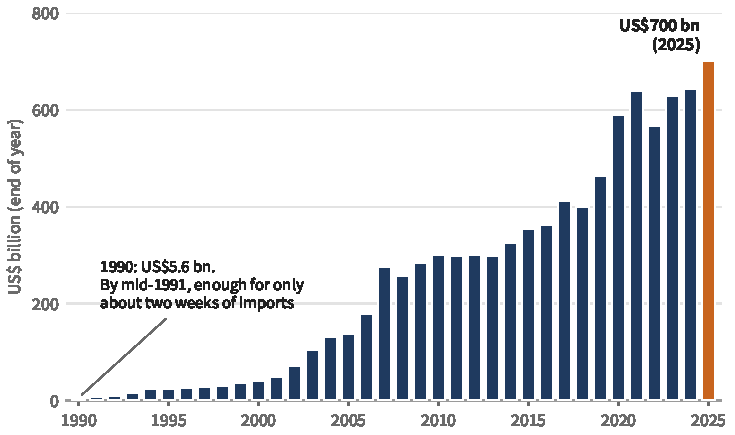
\includegraphics[width=\linewidth]{figures/reserves.pdf}
  \caption{India's foreign exchange reserves, 1990--2025 (US\$ billion, end of year).}
  \label{fig:reserves}
  {\raggedright\small\sffamily Reserves include foreign currency assets, gold, SDRs and the reserve position with the IMF. Notice the dips in 2008 and 2022, partly because the RBI sold dollars to steady the rupee \seesec{sec:moves}.\par}
  \figsource{World Bank (2026b), World Development Indicators, series FI.RES.TOTL.CD.}
\end{figure}

Now let us look at how the RBI uses these reserves to manage the rupee's value. Suppose the rupee is falling too fast against the US dollar, perhaps because too many people are selling rupees to buy dollars. The RBI steps in by selling dollars from its reserves into the foreign exchange market. This \keyterm{intervention}{Buying or selling foreign currency by the central bank to influence the exchange rate.} increases the supply of dollars, making the dollar relatively cheaper and the rupee relatively more valuable, slowing or reversing the rupee's fall (Figure~\ref{fig:intervene}). The opposite happens when the rupee is rising too fast: the RBI buys dollars, increasing demand for the dollar and gently pushing the rupee's value back down.

\begin{figure}[!htb]
  \centering
  % Figure (Section 7, new at merge): how RBI intervention slows a fall in the rupee.
% Demand shifts right by 1 (A ₹85 -> B ₹90); the RBI sells dollars, supply shifts
% right by 0.6 (-> C ₹87). Same geometry as Figures 4 and 10.
\begin{tikzpicture}[ds, x=1.1cm, y=1.1cm]
\draw[ds axis] (0,0) -- (0,3.7) node[above] {₹ per US dollar};
\draw[ds axis] (0,0) -- (5,0);
\node[below] at (2.5,0) {Quantity of US dollars};
\draw[ds demand] (0.4,3.2) -- (3.6,0.6) node[below] {D\textsubscript{0}};
\draw[ds demand, ds new] (1.4,3.2) -- (4.6,0.6) node[below] {D\textsubscript{1}};
\draw[ds supply] (0.4,0.6) -- (3.6,3.2) node[above] {S\textsubscript{0}};
\draw[ds supply, draw=fxteal] (1.0,0.6) -- (4.2,3.2) node[above right=-2pt, text=fxteal, align=left] {S\textsubscript{1}: RBI\\sells dollars};
\draw[ds guide] (0,1.9) -- (2,1.9) -- (2,0);
\draw[ds guide] (0,2.306) -- (2.5,2.306);
\draw[ds guide] (0,2.062) -- (2.8,2.062) -- (2.8,0);
\draw[ds shift] (2.95,1.2) -- (3.75,1.2);
\draw[ds shift, fxteal] (3.12,2.75) -- (3.58,2.75);
\node[ds eq] at (2,1.9) {}; \node[below=3pt] at (2,1.9) {A};
\node[ds eq=fxorange] at (2.5,2.306) {}; \node[above=3pt, text=fxorange] at (2.5,2.306) {\textbf{B}};
\node[ds eq=fxteal] at (2.8,2.062) {}; \node[below right=1pt, text=fxteal] at (2.8,2.062) {\textbf{C}};
\node[left] at (0,1.86) {85};
\node[left, text=fxteal] at (0,2.08) {\textbf{87}};
\node[left, text=fxorange] at (0,2.33) {\textbf{90}};
\end{tikzpicture}

  \caption{How RBI intervention slows a fall in the rupee (hypothetical numbers).}
  \label{fig:intervene}
  {\raggedright\small\sffamily 1. The market starts at A, ₹85 per US dollar. 2. A bigger oil bill shifts demand for dollars right to D\textsubscript{1}. Left alone, the rate would rise to ₹90 at B. 3. The RBI sells dollars from its reserves, so supply shifts right to S\textsubscript{1}. 4. The market settles at C, ₹87: the rupee still falls, but by less, and India's reserves are smaller by the dollars the RBI sold.\par}
  \figsource{Drawn by the authors.}
\end{figure}

However, this tool has clear limits. Foreign exchange reserves, however large, are finite. If strong and sustained market pressure is pushing the rupee in one direction, the RBI cannot fight it indefinitely. This is precisely what happened in 1991, and it is a reminder that while reserves give the RBI significant power to stabilise the currency in the short run, they cannot override fundamental economic forces over the long run \seesec{sec:crises}.
         % Member 3 (was C)
% ============================================================
%  SECTION 8: Nominal and real exchange rates, PPP  (Member 3)
%  Member 3's text. Changes at merge:
%   - Maharaja Mac: undervaluation corrected to about 53 per cent (was "over 40%")
%   - GNI box updated to World Bank 2025 data (Macrotrends source removed)
%   - new figure drawing the worked example
% ============================================================
\section{Nominal and real exchange rates, and purchasing power parity}\label{sec:real}

So far, we have talked about the exchange rate as a single number: how many rupees it takes to buy one US dollar. This is called the \keyterm{nominal exchange rate}{The number of rupees needed to buy one unit of foreign currency, as quoted in the market.}, and it is what you see on a currency exchange board or a news ticker. However, this number alone does not tell the full story of a currency's strength.

Consider this: suppose the nominal exchange rate stays exactly the same, say ₹83 per US dollar, for an entire year. At first glance, nothing has changed. But if prices in India rise by 10 per cent over that year while prices in the US stay flat, Indian goods have become 10 per cent more expensive for American buyers, even though the exchange rate did not move. India has effectively become less competitive as an exporter, not because of any change in the exchange rate, but because of inflation at home. This is what the \keyterm{real exchange rate}{The nominal exchange rate adjusted for differences in price levels between two countries.} captures. It adjusts the nominal rate for differences in price levels between two countries. If Indian prices are rising faster than American prices, the real exchange rate is appreciating even when the nominal rate is unchanged, making Indian exports relatively more expensive.

\begin{workedexample}{How inflation changes the real exchange rate}
Suppose India and the US start the year with an exchange rate of ₹80 per US dollar. India experiences 8 per cent inflation while the US experiences 2 per cent inflation, and the nominal rate stays unchanged.

At the start of the year, a product priced at ₹800 in India costs \$10 in the US. By the end of the year, the same product costs ₹864 in India (up 8 per cent) but only \$10.20 in the US (up 2 per cent). At ₹80 per dollar, ₹864 converts to \$10.80, which is now more expensive than the \$10.20 US price (Figure~\ref{fig:realrate}). Indian exports have become less competitive even though the nominal exchange rate did not change at all. This is what it means for the real exchange rate to appreciate.
\end{workedexample}

\begin{figure}[!htb]
  \centering
  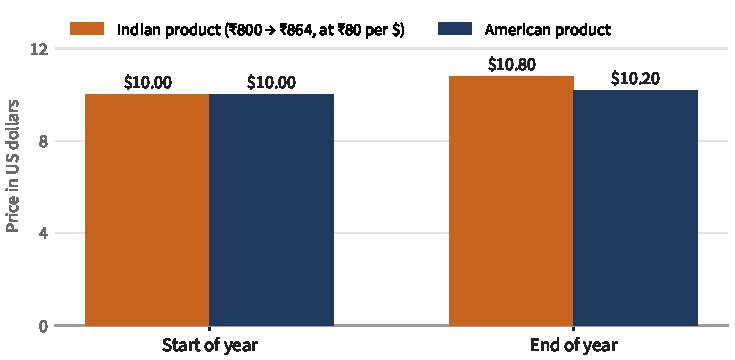
\includegraphics[width=\linewidth]{figures/real_rate.pdf}
  \caption{The same product, priced in dollars, before and after a year of inflation.}
  \label{fig:realrate}
  {\raggedright\small\sffamily The exchange rate stays at ₹80 per US dollar all year. Because prices rise faster in India, the Indian product overtakes its American rival in dollar terms.\par}
  \figsource{Drawn by the authors from the worked example. All values are hypothetical.}
\end{figure}

This idea connects directly to a concept called \keyterm{purchasing power parity (PPP)}{The idea that the same basket of goods should cost the same in every country once prices are converted into one currency.}. PPP is based on a simple idea: a basket of goods should cost the same in every country, once prices are converted into the same currency. If a basket of groceries costs ₹500 in India and \$6 in the US, then the PPP exchange rate would be roughly ₹83 per US dollar. If the actual exchange rate is very different from this, it suggests one currency is overvalued or undervalued.

However, PPP does not hold exactly in the real world. First, transport costs and import taxes mean that identical goods are not equally priced across borders. Second, many goods and services simply cannot be traded across countries at all. A haircut, a local bus ride, or a meal at a street stall in India costs far less than the equivalent in the US, not because of currency misalignment, but because these services are priced according to local wages and cannot be exported to equalise prices.

Despite its limitations, PPP is extremely useful for comparing living standards across countries. If you use the nominal exchange rate to compare incomes, a country with low prices appears poorer than it actually is. PPP adjustments correct for this by accounting for what money can actually buy in each country, giving a fairer picture of real living standards.

\begin{didyouknow}{The Maharaja Mac index}
Every year, \textit{The Economist} magazine publishes the Big Mac index, which compares the price of a McDonald's burger across countries to estimate whether currencies are overvalued or undervalued. Since beef is not widely eaten in India, McDonald's India sells a Maharaja Mac instead, and \textit{The Economist} uses its chicken version as India's entry in the index.

In January 2023, a Maharaja Mac cost ₹207 in India and a Big Mac cost \$5.36 in the US. This implies a PPP exchange rate of about ₹38.6 per US dollar, while the actual rate was around ₹81.7. This suggests the rupee was undervalued by about 53 per cent against the dollar, meaning money goes much further in India than the nominal exchange rate would suggest (The Economist, 2026).
\end{didyouknow}

\begin{didyouknow}{PPP and India's income}
India's nominal gross national income (GNI) per person, converted at market exchange rates, was about \$2,760 in 2025. Adjusted for PPP, it was about \$11,600, roughly 4.2 times higher (World Bank, 2026c). This gap exists because everyday goods and services in India are far cheaper than in high-income countries, so the same amount of money buys much more. International organisations like the World Bank and IMF prefer PPP figures when comparing living standards across countries for exactly this reason.
\end{didyouknow}
         % Member 3 (was 6)
% ============================================================
%  SECTION 9 (was 7): What moves the rupee?        (Member 4)
% ============================================================
\section{What moves the rupee?}\label{sec:moves}

Newspapers report the rupee's movements almost every day: `Rupee falls 30 paise against the dollar'. Behind each such headline sits the model from \secref{sec:ds}. Whenever the rupee moves, ask one question: did something change the demand for dollars, the supply of dollars, or both?

Figure~\ref{fig:history} traces the rupee since 1991. The line climbs from about ₹18 per US dollar to about ₹95, a level first crossed in 2026 (Shivalkar, 2026). Long, quiet stretches are broken by sudden jumps, and each jump has a story behind it.

\begin{figure}[!htb]
  \centering
  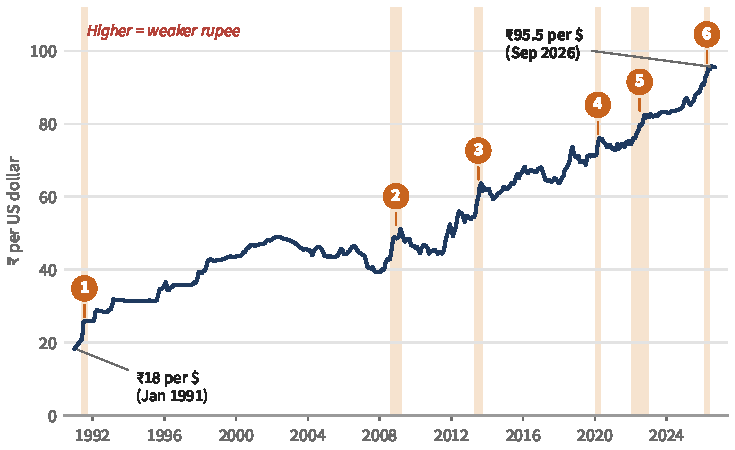
\includegraphics[width=\linewidth]{figures/rupee_history.pdf}
  \caption{The rupee against the US dollar, January 1991 to September 2026.}
  \label{fig:history}
  {\raggedright\small\sffamily Each point is the average exchange rate for one month. A rise in the line means it takes more rupees to buy one dollar, so the rupee has weakened. The shaded bands, numbered 1 to 6, mark six sharp falls in the rupee. The box `Reading the rupee's history' asks you to identify them.\par}
  \figsource{Board of Governors of the Federal Reserve System (2026a), series EXINUS, monthly averages, retrieved from FRED, 1 November 2026.}
\end{figure}

The slow part of the climb is mainly about inflation. Prices in India have usually risen faster than in the United States, which slowly makes Indian goods dearer for foreign buyers and American goods cheaper for Indians \seesec{sec:real}. Fewer dollars come in through exports, more are needed for imports, and the rupee drifts down year after year.

The sudden jumps are usually about money crossing borders. When foreigners buy Indian shares, bonds or businesses, dollars flow in; when they sell, dollars flow out. These movements are called \keyterm{capital flows}{Money that moves between countries to buy or sell financial assets, such as shares and bonds, or real assets, such as factories.}. Portfolio money is the quickest to leave \seesec{sec:forex}, which is why it matters so much for short-run swings.

What makes this money move? Very often, interest rates. Investors compare what they can earn on an American government bond with what they can earn on an Indian one. The gap between the two is the \keyterm{interest rate differential}{The difference between the interest rates paid in two countries. Funds tend to move towards the higher return, after allowing for risk.}. When the US Federal Reserve raises its interest rate, the gap narrows. Foreign investors sell Indian assets and take their dollars home, and the supply of dollars shifts to the left (Figure~\ref{fig:shocks}b). This is why a decision taken in Washington is front-page news in Mumbai.

Crude oil is the other big mover. India imports about 88 per cent of the crude oil it uses (Petroleum Planning \& Analysis Cell [PPAC], 2025). When the world price of oil rises, refiners need more dollars to buy the same number of barrels, and the demand for dollars shifts to the right (Figure~\ref{fig:shocks}a). A widening current account deficit \seesec{sec:bop} has a similar effect.

\begin{figure}[!htb]
  \centering
  \resizebox{0.92\linewidth}{!}{% Figure (Section 9, Member 4): two shocks in the market for US dollars.
% (a) oil price rise: demand shifts right, ₹85 -> ₹90.
% (b) US interest rates rise: supply shifts left, ₹85 -> ₹89.
% Same geometry as Figure 4: D: y = 3.2 - 0.8125(x - 0.4), S: y = 0.6 + 0.8125(x - 0.4).
\begin{tikzpicture}[ds, x=0.9cm]
\foreach \ox/\title in {0/{(a) World oil price rises}, 6.2/{(b) US interest rates rise}} {
  \begin{scope}[shift={(\ox,0)}]
    \draw[ds axis] (0,0) -- (0,3.7) node[above] {₹ per US dollar};
    \draw[ds axis] (0,0) -- (5,0);
    \node[below] at (2.5,0) {Quantity of US dollars};
    \node[ds title] at (-0.4,4.15) {\title};
  \end{scope}
}
% (a) demand shifts right by 1: E1 at (2.5, 2.306)
\draw[ds demand] (0.4,3.2) -- (3.6,0.6) node[below] {D\textsubscript{0}};
\draw[ds demand, ds new] (1.4,3.2) -- (4.6,0.6) node[below] {D\textsubscript{1}};
\draw[ds supply] (0.4,0.6) -- (3.6,3.2) node[above] {S};
\draw[ds shift] (2.95,1.2) -- (3.75,1.2);
\draw[ds guide] (0,1.9) -- (2,1.9) -- (2,0);
\draw[ds guide] (0,2.306) -- (2.5,2.306) -- (2.5,0);
\node[ds eq] at (2,1.9) {}; \node[below=3pt] at (2,1.9) {E\textsubscript{0}};
\node[ds eq=fxgreen] at (2.5,2.306) {}; \node[above=3pt, text=fxgreen] at (2.5,2.306) {\textbf{E\textsubscript{1}}};
\node[left] at (0,1.9) {85};
\node[left, text=fxgreen] at (0,2.306) {\textbf{90}};
% (b) supply shifts left by 0.8: E1 at (1.6, 2.225)
\begin{scope}[shift={(6.2,0)}]
  \draw[ds demand] (0.4,3.2) -- (3.6,0.6) node[below] {D};
  \draw[ds supply] (0.4,0.6) -- (3.6,3.2) node[above] {S\textsubscript{0}};
  \draw[ds supply, ds new] (0,0.925) -- (2.8,3.2) node[above] {S\textsubscript{1}};
  \draw[ds shift] (2.9,2.7) -- (2.28,2.7);
  \draw[ds guide] (0,1.9) -- (2,1.9) -- (2,0);
  \draw[ds guide] (0,2.225) -- (1.6,2.225) -- (1.6,0);
  \node[ds eq] at (2,1.9) {}; \node[right=5pt] at (2,1.9) {E\textsubscript{0}};
  \node[ds eq=fxgreen] at (1.6,2.225) {}; \node[above=3pt, text=fxgreen] at (1.6,2.225) {\textbf{E\textsubscript{1}}};
  \node[left] at (0,1.9) {85};
  \node[left, text=fxgreen] at (0,2.225) {\textbf{89}};
\end{scope}
\end{tikzpicture}
}
  \caption{Two shocks in the market for US dollars (hypothetical numbers).}
  \label{fig:shocks}
  {\raggedright\small\sffamily (a) 1. The market starts at E\textsubscript{0}, ₹85 per dollar. 2. Oil now costs more, so refiners want more dollars at every exchange rate: demand shifts right to D\textsubscript{1}. 3. At ₹85 there is excess demand for dollars, and buyers bid the price up. 4. The new equilibrium E\textsubscript{1} is at ₹90: the rupee has depreciated and more dollars change hands.\\
  (b) 1. Start again at E\textsubscript{0}, ₹85. 2. Foreign investors move funds to the United States, so fewer dollars are offered in India at every exchange rate: supply shifts left to S\textsubscript{1}. 3. The new equilibrium E\textsubscript{1} is at ₹89: the rupee has depreciated and fewer dollars change hands.\par}
  \figsource{Drawn by the authors.}
\end{figure}

Markets also look ahead. If traders expect the rupee to fall, importers rush to buy dollars today and exporters hold on to the dollars they already have. Buying or selling a currency to profit from its expected future price is called \keyterm{speculation}{Buying or selling an asset, such as a currency, in the hope of profiting from a change in its price.}. It can turn a fear into a fact: the rupee falls partly because so many people acted on the belief that it would.

Real episodes usually mix several of these forces. In the global financial crisis of 2008 and the COVID-19 panic of 2020, investors everywhere fled to the safety of the US dollar. India caused neither crisis, yet the rupee fell both times. Table~\ref{tab:moves} sums up the forces, and the box that follows asks you to read the rupee's history for yourself.

\begin{table}[!htb]
\centering\small\sffamily
\caption{What moves the rupee: a summary.}\label{tab:moves}
\begin{tabularx}{\linewidth}{@{}>{\raggedright\arraybackslash}p{38mm}>{\raggedright\arraybackslash}X>{\raggedright\arraybackslash}p{12mm}>{\raggedright\arraybackslash}p{18mm}@{}}
\toprule
\textbf{What happens} & \textbf{Effect in the market for dollars} & \textbf{₹/\$ rate} & \textbf{Rupee}\\
\midrule
Inflation in India runs ahead of US inflation & Demand rises and supply falls, slowly, over years & Rises & Depreciates\\
US interest rates rise & Supply shifts left as foreign investors take money home & Rises & Depreciates\\
Foreign investors pour money into India & Supply shifts right & Falls & Appreciates\\
World crude oil price rises & Demand shifts right & Rises & Depreciates\\
Current account deficit widens & Demand for dollars runs ahead of supply from trade & Rises & Depreciates\\
Traders expect the rupee to fall & Demand shifts right and supply shifts left & Rises & Depreciates\\
Global panic (`flight to safety') & Supply shifts left as money leaves emerging economies & Rises & Depreciates\\
\bottomrule
\end{tabularx}
\par\smallskip{\raggedright\footnotesize\sffamily\color{fxmuted}Each change is assumed to happen on its own, with everything else held constant. The opposite change has the opposite effect.\par}
\end{table}

\begin{economistsfacts}{Reading the rupee's history}
Figure~\ref{fig:history} marks six sharp jumps in the price of the dollar, numbered 1 to 6. Each matches one of the events below, which are listed in no particular order.
\begin{enumerate}[label=\Alph*., leftmargin=1.6em]
  \item The US Federal Reserve raises interest rates at its fastest pace in four decades, while war in Ukraine pushes up oil prices.
  \item India, with reserves for only about two weeks of imports, devalues the rupee.
  \item Conflict in West Asia sends crude oil above \$110 a barrel, and foreign investors sell Indian assets.
  \item A giant American investment bank collapses and a global financial crisis spreads.
  \item The US central bank hints that it will soon slow its support for the American economy, and investors pull money out of emerging markets.
  \item A new virus shuts down economies around the world.
\end{enumerate}
\textbf{1.} Match each number to an event. \textbf{2.} For each, say whether the main change was in the demand for dollars, the supply of dollars, or both. \textbf{3.} One event does not fit the demand-and-supply story. Which one, and why? (Hint: see \secref{sec:systems}.)
\answers{1--B (1991): does not fit, because the rate was cut by an official devaluation, not by the market. 2--D (2008): supply shifted left as investors fled to the dollar. 3--E (2013, the `taper tantrum'): supply shifted left as foreign money left; India's large current account deficit kept demand high. 4--F (2020): supply shifted left in a global flight to safety. 5--A (2022): both, supply left (US rate rises) and demand right (dearer oil). 6--C (2026): both, demand right (oil) and supply left (foreign investors sold Indian assets).}
\end{economistsfacts}
       % Member 4 (was 7)
% ============================================================
%  SECTION 10 (was 8): Why exchange rates matter for India   (Member 4)
%  Selvi box changed at merge to ₹90 -> ₹95 to match Member 1's ₹95.
% ============================================================
\section{Why exchange rates matter for India}\label{sec:matters}

You have already met the winners and losers from a change in the rupee \seesec{sec:appdep}. Here we follow those effects through the wider economy. Whether you gain or lose depends on whether you earn dollars, spend them or owe them.

Start with those who earn dollars. When the rupee weakens, every dollar an exporter earns turns into more rupees. The exporter can keep the dollar price unchanged and enjoy a bigger income, or cut the price abroad to win more orders. Either way, Indian goods become easier to sell, and we say that their \keyterm{export competitiveness}{The ability of a country's firms to sell goods and services abroad at prices that foreign buyers are willing to pay.} has improved. The gain is smaller than it looks for firms that import their own raw materials or machines, as the story of Selvi's unit shows.

\begin{casestudy}{A weaker rupee in Selvi's unit}
Selvi's unit in Tiruppur sells cotton T-shirts to a buyer in the United States, priced in dollars. Last year she shipped an order worth \$20,000 when the rupee was at ₹90 per dollar, and it brought in ₹18 lakh. This year the same order, at ₹95, brings in ₹19 lakh. The extra ₹1 lakh can pay for overtime wages, or let her offer a small discount to win the next order.

This is not just a classroom story. In early 2025, the Tiruppur Exporters' Association estimated that the rupee's fall during 2024 accounted for about 5 per cent of the growth in the town's garment exports (Business Standard, 2025a).

But Selvi's gain is not pure profit. Some of her dyes, accessories and machine parts are imported, and these now cost more. Her American buyer reads the same news, too, and may ask her to share the gain through a lower price. And if the rupee turns and strengthens, the gain disappears; that is exactly the risk her forward contract guards against \seesec{sec:forex}.
\figsource{The order values and exchange rates in this example are hypothetical.}
\end{casestudy}

Now consider those who spend dollars. India imports crude oil, gold, electronics, fertiliser and edible oil, almost all priced in dollars. A weaker rupee makes each of them dearer in rupees, even when the dollar price has not changed. Diesel runs the trucks that carry vegetables, grain and medicines, so costlier fuel spreads into the price of almost everything (Figure~\ref{fig:inflation}). A rise in prices that comes from dearer imports is called \keyterm{imported inflation}{A rise in the general price level caused by higher rupee prices of imported goods, often because the rupee has depreciated.}.

\begin{figure}[!htb]
  \centering
  \resizebox{\linewidth}{!}{% Figure (Section 10, Member 4): how a weaker rupee turns into imported inflation.
% Same look as Member 1's flow diagram (Figure 2).
\begin{tikzpicture}[
  font=\sffamily\small,
  chainbox/.style={fill=fxnavy!8, draw=fxnavy, line width=0.8pt, rounded corners=1.5mm,
               text width=24mm, minimum height=19mm, align=center, inner sep=3pt},
  last/.style={chainbox, fill=fxorange, draw=fxorange, text=white},
  flow/.style={-{Stealth[length=2.6mm,width=2.2mm]}, line width=1.3pt, fxnavy},
  node distance=5mm,
]
\node[chainbox] (a) {\textbf{Rupee weakens}\\[2pt]{\footnotesize ₹85 → ₹90 per US dollar}};
\node[chainbox, right=of a] (b) {\textbf{Imports cost more}\\[2pt]{\footnotesize crude oil, edible oil, electronics, fertiliser}};
\node[chainbox, right=of b] (c) {\textbf{Fuel prices rise}\\[2pt]{\footnotesize petrol, diesel and LPG}};
\node[chainbox, right=of c] (d) {\textbf{Costs rise}\\[2pt]{\footnotesize transport and production}};
\node[last, right=of d] (e) {\textbf{Prices rise}\\[2pt]{\footnotesize food and everyday goods: imported inflation}};
\foreach \u/\v in {a/b, b/c, c/d, d/e} \draw[flow] (\u) -- (\v);
\end{tikzpicture}
}
  \caption{How a weaker rupee becomes imported inflation.}
  \label{fig:inflation}
  {\raggedright\small\sffamily Read the chain from left to right. Each step takes time, so the full effect on prices can take several months to appear. The exchange rates shown are hypothetical.\par}
  \figsource{Drawn by the authors.}
\end{figure}

\begin{workedexample}{The same barrel, a different price}
Suppose a barrel of crude oil costs \$80 on the world market (hypothetical figures).
\begin{itemize}
  \item At ₹85 per US dollar, India pays 80 × 85 = ₹6,800 per barrel.
  \item At ₹90 per US dollar, India pays 80 × 90 = ₹7,200 per barrel.
\end{itemize}
The oil has not become any dearer in dollars, yet India pays ₹400 more for every barrel, a rise of about 5.9 per cent.

\textbf{Now you try.} The dollar price of oil rises to \$90 while the rupee stays at ₹90 per dollar. What is the new rupee price of a barrel, and by what percentage has it risen compared with ₹6,800?
\answers{₹8,100, a rise of about 19 per cent. When oil prices rise and the rupee weakens together, the two effects multiply.}
\end{workedexample}

Then there are those who owe dollars. A company that borrowed in dollars, such as an airline paying for new aircraft, must now find more rupees to repay the same loan. A sharp fall in the rupee can turn a healthy balance sheet into a worrying one.

All of this matters to the Reserve Bank of India. When the RBI raises its policy interest rate (the repo rate), Indian assets pay more, foreign money tends to flow in and the rupee strengthens. Imports become cheaper and inflation cools, although exporters find life harder. This route from interest rates to spending and prices, working through the exchange rate, is called the \keyterm{exchange rate channel}{The way a change in the central bank's policy interest rate affects spending and prices by moving the exchange rate, and through it exports and imports.} of monetary policy (Jayadev, 2021, Section 15.9). It is one reason the RBI keeps a close eye on the rupee whenever it sets interest rates.
      % Member 4 (was 8)
% ============================================================
%  SECTION 11 (was D): When currencies collapse     (Member 4)
%  At merge: 1991 wording and devaluation size aligned with Section 6;
%  India's reserves aligned with Section 7 (RBI, 2026c).
% ============================================================
\section{When currencies collapse: crises in South Asia}\label{sec:crises}

Foreign exchange reserves work like a family's savings for a bad year \seesec{sec:reserves}. But what happens when the savings run out? A country that cannot find enough dollars to pay for its imports and repay its foreign loans can no longer protect its currency. The result is a \keyterm{currency crisis}{A sudden and large fall in the value of a country's currency, usually because the country has run short of foreign exchange.}: a sudden, steep fall in the value of a currency, usually together with shortages and soaring prices. Two of India's neighbours have lived through one recently.

\minihead{Sri Lanka, 2022.} Sri Lanka's troubles built up over several years. Large tax cuts in 2019 reduced the government's income. The COVID-19 pandemic then emptied the tourist hotels that had earned much of the country's foreign currency, while big repayments on foreign loans kept falling due. The central bank held the Sri Lankan rupee at about 200 per dollar and spent its reserves to do so. By the end of March 2022, gross reserves were down to about US\$1.9 billion, and most of that could not easily be spent (Daily Mirror, 2022).

Once the currency was allowed to float in March 2022, it crashed, from about 202 rupees per dollar in February to about 356 by May (Figure~\ref{fig:srilanka}). Fuel, cooking gas and medicines ran short, and people queued for hours outside petrol pumps. In April 2022 the government stopped paying its foreign debts, Sri Lanka's first \keyterm{sovereign default}{When a government fails to make the payments on its debt that it has promised.}. Inflation reached 69.8 per cent in September 2022 (Central Bank of Sri Lanka [CBSL], 2022). In March 2023 the IMF approved a loan of about US\$3 billion (International Monetary Fund [IMF], 2023a), and prices slowly began to settle.

\begin{figure}[!htb]
  \centering
  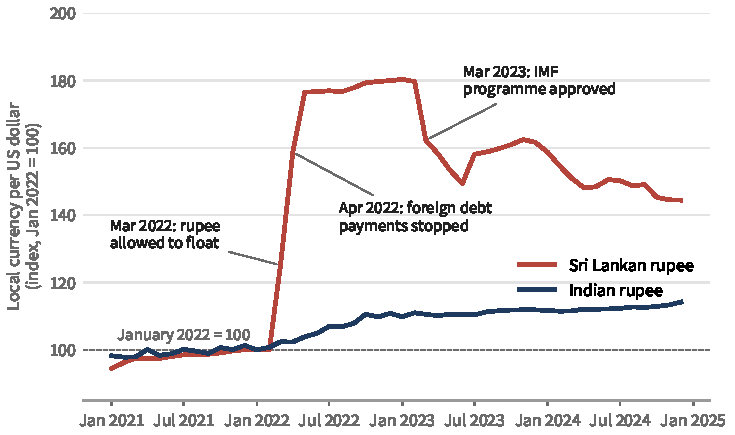
\includegraphics[width=\linewidth]{figures/srilanka_index.pdf}
  \caption{The Sri Lankan and Indian rupees against the US dollar, 2021 to 2024.}
  \label{fig:srilanka}
  {\raggedright\small\sffamily Both lines show how many units of local currency it takes to buy one dollar, scaled so that January 2022 = 100. A rise means the currency has weakened. Once Sri Lanka stopped defending its rupee, it lost value within weeks. The Indian rupee also weakened over 2022, but gradually.\par}
  \figsource{Board of Governors of the Federal Reserve System (2026a, 2026b), series EXINUS and EXSLUS, monthly averages, retrieved from FRED, 1 November 2026. Index calculated by the authors.}
\end{figure}

\minihead{Pakistan, 2022--23.} Pakistan came close to the same edge. High oil prices widened its current account deficit, floods in the summer of 2022 destroyed crops and homes, and talks with the IMF stalled. In early February 2023, the State Bank of Pakistan's reserves fell to about US\$2.9 billion, their lowest level in nine years and barely enough for a few weeks of imports (Business Recorder, 2023a). The government restricted imports and the Pakistani rupee slid, reaching a record low of about 307 per dollar in September 2023 (Xinhua, 2023). Inflation hit 38 per cent in May 2023 (Business Recorder, 2023b). A US\$3 billion \keyterm{IMF programme}{A loan from the International Monetary Fund to a country short of foreign currency, paid in instalments on condition that the country carries out agreed policy changes.}, approved in July 2023, helped Pakistan avoid default (IMF, 2023b).

\minihead{What about India?} Both stories echo India's own crisis of 1991 \seesec{sec:systems}, when reserves covered only about two weeks of imports. India's position today is much stronger. Its reserves stood at about US\$682 billion in May 2026, enough for about 11 months of imports (RBI, 2026c). Under a managed float, the rupee adjusts a little every day, so pressure is released gradually instead of building up behind a fixed rate. And earnings from software services and remittances cover a large part of the gap in goods trade \seesec{sec:bop}.

\begin{table}[!htb]
\centering\small\sffamily
\caption{Three currency crises compared.}\label{tab:crises}
\begin{tabularx}{\linewidth}{@{}>{\raggedright\arraybackslash}p{24mm}>{\raggedright\arraybackslash}X>{\raggedright\arraybackslash}X>{\raggedright\arraybackslash}X@{}}
\toprule
 & \textbf{India, 1991} & \textbf{Sri Lanka, 2022} & \textbf{Pakistan, 2022--23}\\
\midrule
\textbf{Main triggers} & Oil price spike during the Gulf War; fall in remittances; large fiscal and current account deficits & Tax cuts; collapse of tourism during COVID-19; heavy foreign debt repayments; a sudden ban on chemical fertilisers that hurt harvests & High oil prices; large current account deficit; 2022 floods; political uncertainty; stalled IMF talks\\
\addlinespace
\textbf{Reserves at the worst point} & About two weeks of imports & About US\$1.9 billion (March 2022) & About US\$2.9 billion (February 2023)\\
\addlinespace
\textbf{What happened to the currency} & Devalued by about 18--20 per cent in two steps (1--3 July 1991) & Fell from about 202 to about 356 per dollar within three months of floating & Slid to a record low of about 307 per dollar (September 2023)\\
\addlinespace
\textbf{Peak inflation} & 13.7\% (1991--92, wholesale prices) & 69.8\% (September 2022) & 38\% (May 2023)\\
\addlinespace
\textbf{The way out} & IMF loan, gold pledged abroad and wide-ranging economic reforms & Default on foreign debt (April 2022); IMF programme of about US\$3 billion (March 2023); debt restructuring & IMF Stand-By Arrangement of US\$3 billion (July 2023); curbs on imports\\
\bottomrule
\end{tabularx}
\figsource{Business Recorder (2023a, 2023b); CBSL (2022); Daily Mirror (2022); IMF (2023a, 2023b); Xinhua (2023); RBI (n.d.) and Section~\ref{sec:systems} for India, 1991.}
\end{table}

The lesson from all three cases is that currencies rarely collapse because of a single bad event. Low reserves, heavy foreign-currency debt and a large current account deficit are like dry wood. A pandemic, an oil shock or a flood only supplies the spark.

\begin{economistsdisagree}{Is the IMF's medicine too bitter?}
IMF loans come with conditions. Under its 2023 programme, for example, Sri Lanka agreed to raise taxes and to price fuel and electricity so that they cover their costs.

Supporters argue that the conditions fix the problems that caused the crisis in the first place. They also reassure other lenders and investors, who return only when they trust the government's plans. Without reform, they say, the loan would simply be spent and the crisis would return.

Critics reply that raising taxes and cutting spending in the middle of a crisis makes the slump deeper. The burden falls hardest on poor families, who spend most of their income on food and fuel. And conditions drawn up in Washington may not suit local circumstances.

What do you think? Should help in a crisis come with strings attached?
\end{economistsdisagree}
           % Member 4 (was D)
% ============================================================
%  CONCLUSION (end of chapter)                    (Member 1)
% ============================================================
\section*{Conclusion}
\addcontentsline{toc}{section}{Conclusion}

Now look again at Meera's fees. In 2026, dearer oil raised India's demand for dollars, while foreign investors selling Indian assets cut the supply \seesec{sec:moves}. The RBI sold dollars from its reserves to slow the rupee's fall but did not stop it, and the bill for her fees went up by ₹2.5 lakh. The same move gave Ravi's family more rupees for every dirham. An exchange rate is just a price, but so much of India's trade, savings and borrowing passes through it that this one price reaches almost every household in the country.

% [added at merge] summary box answering the five questions from the Introduction
\begin{keypoints}[unbreakable]{What this chapter has shown}
\begin{itemize}
  \item \textbf{Why a currency has a price.} When goods, services or savings cross a border, one currency must be swapped for another. The exchange rate is the price of that swap (Section~\ref{sec:exrate}).
  \item \textbf{Who buys and sells currencies.} Importers, students abroad and Indians investing abroad demand dollars; exporters, workers abroad, foreign tourists and foreign investors supply them, through banks regulated by the RBI (Sections~\ref{sec:forex} and~\ref{sec:bop}).
  \item \textbf{What sets the price, and why it keeps changing.} The demand for and supply of dollars. Inflation, interest rates, capital flows, oil prices and expectations keep shifting the two curves (Sections~\ref{sec:ds}, \ref{sec:real} and~\ref{sec:moves}).
  \item \textbf{How it is managed.} Countries choose fixed, floating or managed rates. Since 1993 India has used a managed float, with the RBI using its reserves to smooth sharp swings, though no country's reserves can hold a rate for ever (Sections~\ref{sec:systems}, \ref{sec:reserves} and~\ref{sec:crises}).
  \item \textbf{Who gains and who loses.} A weaker rupee helps exporters and families receiving remittances, but hurts importers, students abroad and anyone with dollar debts, and it can push up prices at home (Sections~\ref{sec:appdep} and~\ref{sec:matters}).
\end{itemize}
\textbf{Where next?} The balance of payments, monetary policy and international trade each build on the ideas in this chapter.
\end{keypoints}
       % Member 1

\clearpage
% Generated by source/build_book.py from the \keyterm definitions. Do not edit by hand.
\section*{Glossary}
\addcontentsline{toc}{section}{Glossary}
\begingroup\small\setlength{\parindent}{-1.5em}\setlength{\leftskip}{1.5em}\RaggedRight
\textbf{appreciation}\quad A rise in the value of a currency set by the market; here, fewer rupees are needed to buy one dollar.\par\smallskip
\textbf{authorised dealers}\quad Banks and firms licensed by the RBI under FEMA, 1999, to buy and sell foreign currency.\par\smallskip
\textbf{balance of payments (BoP)}\quad The record of all economic transactions between a country's residents and the rest of the world over a period.\par\smallskip
\textbf{capital account}\quad The part of the BoP that records the buying and selling of assets, such as FDI, FPI and loans.\par\smallskip
\textbf{capital flows}\quad Money that moves between countries to buy or sell financial assets, such as shares and bonds, or real assets, such as factories.\par\smallskip
\textbf{currency crisis}\quad A sudden and large fall in the value of a country's currency, usually because the country has run short of foreign exchange.\par\smallskip
\textbf{current account}\quad The part of the BoP that records trade in goods and services, income and transfers.\par\smallskip
\textbf{current account deficit (CAD)}\quad The gap when a country's payments abroad for goods, services, income and transfers exceed its receipts.\par\smallskip
\textbf{demand for foreign exchange}\quad The foreign currency that residents want, to pay for imports, study and travel abroad, investment abroad and foreign loans.\par\smallskip
\textbf{depreciation}\quad A fall in the value of a currency set by the market; here, more rupees are needed to buy one dollar.\par\smallskip
\textbf{devaluation}\quad A deliberate cut in a currency's official value by the government or central bank under a fixed exchange rate.\par\smallskip
\textbf{direct quote}\quad The price of one unit of foreign currency in home currency, e.g.\ US\$1 = ₹95.\par\smallskip
\textbf{equilibrium exchange rate}\quad The exchange rate at which the quantity of dollars demanded equals the quantity supplied.\par\smallskip
\textbf{excess demand}\quad When buyers want more dollars than are on offer at the current exchange rate; the rate tends to rise.\par\smallskip
\textbf{excess supply}\quad When more dollars are offered than buyers want at the current exchange rate; the rate tends to fall.\par\smallskip
\textbf{exchange rate}\quad The price of one currency in terms of another, for example ₹95 per US dollar.\par\smallskip
\textbf{exchange rate channel}\quad The way a change in the central bank's policy interest rate affects spending and prices by moving the exchange rate, and through it exports and imports.\par\smallskip
\textbf{exchange rate system}\quad The rules a country follows to manage the value of its currency against other currencies.\par\smallskip
\textbf{export competitiveness}\quad The ability of a country's firms to sell goods and services abroad at prices that foreign buyers are willing to pay.\par\smallskip
\textbf{fixed (pegged) exchange rate}\quad An exchange rate held at a set value against another currency, a basket of currencies or gold by the central bank.\par\smallskip
\textbf{floating (flexible) exchange rate}\quad An exchange rate set by demand and supply in the market, with little government control.\par\smallskip
\textbf{foreign direct investment (FDI)}\quad Buying a lasting stake (10\% or more) in a business abroad, or setting one up.\par\smallskip
\textbf{foreign exchange market}\quad The market in which currencies are traded for one another. Also called the forex market.\par\smallskip
\textbf{foreign exchange reserves}\quad Foreign currency assets, gold and other reserve assets held by the RBI on behalf of the country.\par\smallskip
\textbf{foreign portfolio investment (FPI)}\quad Buying shares and bonds (holdings under 10\%), which can be sold quickly.\par\smallskip
\textbf{iMF programme}\quad A loan from the International Monetary Fund to a country short of foreign currency, paid in instalments on condition that the country carries out agreed policy changes.\par\smallskip
\textbf{import cover}\quad The number of months of imports a country could pay for using only its reserves.\par\smallskip
\textbf{imported inflation}\quad A rise in the general price level caused by higher rupee prices of imported goods, often because the rupee has depreciated.\par\smallskip
\textbf{indirect quote}\quad How much foreign currency one unit of home currency buys, e.g.\ ₹1 = US\$0.0105.\par\smallskip
\textbf{interest rate differential}\quad The difference between the interest rates paid in two countries. Funds tend to move towards the higher return, after allowing for risk.\par\smallskip
\textbf{intervention}\quad Buying or selling foreign currency by the central bank to influence the exchange rate.\par\smallskip
\textbf{invisibles}\quad Trade in services, income and transfers, as opposed to trade in goods.\par\smallskip
\textbf{managed float}\quad An exchange rate mainly set by the market, with the central bank stepping in to prevent sharp swings.\par\smallskip
\textbf{nominal exchange rate}\quad The number of rupees needed to buy one unit of foreign currency, as quoted in the market.\par\smallskip
\textbf{purchasing power parity (PPP)}\quad The idea that the same basket of goods should cost the same in every country once prices are converted into one currency.\par\smallskip
\textbf{real exchange rate}\quad The nominal exchange rate adjusted for differences in price levels between two countries.\par\smallskip
\textbf{remittances}\quad Money that people working abroad send home to their families.\par\smallskip
\textbf{revaluation}\quad A deliberate increase in a currency's official value under a fixed exchange rate.\par\smallskip
\textbf{sovereign default}\quad When a government fails to make the payments on its debt that it has promised.\par\smallskip
\textbf{Special Drawing Rights (SDR)}\quad An international reserve asset created by the IMF that member countries can use to settle payments with each other.\par\smallskip
\textbf{speculation}\quad Buying or selling an asset, such as a currency, in the hope of profiting from a change in its price.\par\smallskip
\textbf{supply of foreign exchange}\quad The foreign currency flowing into a country from its exports, remittances, tourists and foreign investment.\par\smallskip
\endgroup

% ============================================================
%  END-OF-CHAPTER QUESTIONS
%  Sections 1-3: Member 1's questions. Sections 9-11: Member 4's.
%  Sections 4-8: written at merge (Members 2 and 3 did not supply questions).
% ============================================================
\section*{Review questions}
\addcontentsline{toc}{section}{Review questions}
\begingroup\small
\newcommand{\qsec}[1]{\par\medskip{\sffamily\bfseries\color{fxnavy}#1}\par}
\newcommand{\ans}[1]{\par{\color{fxmuted}\footnotesize\sffamily\textbf{Answer.} #1}\par\smallskip}

\qsec{Sections 1--3: Exchange rates, the forex market and the balance of payments}
\begin{enumerate}[leftmargin=1.6em, label=\arabic*., itemsep=3pt]
\item The rate moves from ₹90 to ₹95 per US dollar. Has the rupee become stronger or weaker? Explain.
\ans{Weaker. Each dollar now costs more rupees, so each rupee buys fewer dollars.}
\item Write the direct quote ``US\$1 = ₹80'' as an indirect quote.
\ans{₹1 = US\$0.0125 (1 ÷ 80).}
\item A money changer buys dollars at ₹94 and sells them at ₹96. What is the spread on US\$100?
\ans{₹200 (₹9,600 − ₹9,400).}
\item Give two sources of demand for dollars and two sources of supply of dollars in India.
\ans{Demand: importers of oil or gold, students paying foreign fees, Indian tourists abroad, Indians investing abroad. Supply: exporters, remittances, foreign tourists in India, FDI and FPI inflows.}
\item Why does a fall in the rupee against the dollar mean more rupees for Ravi, even though he is paid in dirhams?
\ans{The dirham is fixed at 3.6725 per US dollar. When the dollar costs more rupees, so does the dirham.}
\item What is the difference between FDI and FPI, and which is more likely to cause sudden moves in the rupee?
\ans{FDI buys a lasting stake in a business and stays for years. FPI buys shares and bonds and can leave in a day. FPI is more likely to cause sudden moves.}
\item Why might Selvi sign a forward contract?
\ans{To fix today the rate at which she will sell her dollars later, so that a stronger rupee does not wipe out her profit.}
\item India imports far more goods than it exports. Why is its current account deficit still small?
\ans{Large net earnings from invisibles, mainly software exports and remittances, cover most of the trade gap.}
\item How can a country pay for a current account deficit?
\ans{With a net inflow on the capital account (such as FDI, FPI or loans) or by drawing down its foreign exchange reserves.}
\end{enumerate}

\qsec{Sections 4--8: How the rate is set and managed}
\begin{enumerate}[resume, leftmargin=1.6em, label=\arabic*., itemsep=3pt]
\item At ₹80 per US dollar, buyers want US\$120 million and sellers offer US\$100 million. Is there excess demand or excess supply, and which way will the rate move?
\ans{Excess demand of US\$20 million. Buyers bid the rate up, so the rupee depreciates until the two quantities are equal.}
\item What is the difference between a depreciation and a devaluation? Give one Indian example of a devaluation.
\ans{A depreciation is a fall in a market-set rate; a devaluation is a deliberate cut in an official, fixed rate. India devalued the rupee in June 1966 (to ₹7.50 per dollar) and in July 1991.}
\item Name the three main types of exchange rate system. Which one has India used since March 1993?
\ans{Fixed (pegged), floating (flexible) and managed float. India has used a managed float since 1993.}
\item Draw a demand-and-supply diagram to show how the RBI can slow a fall in the rupee. What happens to India's reserves?
\ans{Supply of dollars shifts right as the RBI sells dollars, so the rate rises by less than it otherwise would (as in Figure~\ref{fig:intervene}). Reserves fall by the dollars sold.}
\item A pair of shoes costs ₹2,400 in India and \$40 in the US. What PPP exchange rate does this imply? If the market rate is ₹95 per dollar, is the rupee overvalued or undervalued by this measure?
\ans{₹60 per dollar (2,400 ÷ 40). At ₹95 a dollar buys more in India than PPP suggests, so the rupee is undervalued.}
\end{enumerate}

\qsec{Sections 9--11: What moves the rupee, why it matters, and crises}
\begin{enumerate}[resume, leftmargin=1.6em, label=\arabic*., itemsep=3pt]
\item The US Federal Reserve raises its interest rate sharply. Assuming nothing else changes, what is most likely to happen in the market for US dollars in India?\\
(a) The demand curve for dollars shifts left and the rupee appreciates.\\
(b) The supply curve of dollars shifts left and the rupee depreciates.\\
(c) The supply curve of dollars shifts right and the rupee appreciates.\\
(d) Nothing changes, because the RBI has not changed its own interest rate.
\ans{(b). The interest rate differential narrows, so foreign investors move funds out of India. Fewer dollars are offered at every exchange rate, and the ₹/\$ rate rises.}
\item Which of the following is an example of imported inflation?\\
(a) Vegetable prices rise after a weak monsoon.\\
(b) Diesel prices rise after the rupee falls from ₹85 to ₹90 per US dollar.\\
(c) House rents rise in Bengaluru as more IT firms open offices.\\
(d) Wages rise after a new minimum wage law.
\ans{(b). Only (b) starts with imports becoming dearer in rupees. The others are caused by domestic supply or demand conditions.}
\item In 2022, world crude oil prices rose and the US Federal Reserve raised interest rates at the same time. (i) Draw a diagram of the market for US dollars in India showing both changes. (ii) Explain why we can be sure what happened to the value of the rupee, but not to the quantity of dollars traded.
\ans{(i) Demand for dollars shifts right (refiners need more dollars for oil); supply shifts left (foreign investors take funds to the US). (ii) Both shifts push the ₹/\$ rate up, so the rupee clearly depreciates. The demand shift raises the quantity traded while the supply shift lowers it, so the net effect on quantity depends on which shift is larger.}
\item Which combination of conditions left Sri Lanka most exposed to a currency crisis in 2022?\\
(a) High reserves, little foreign debt and a booming tourism sector.\\
(b) Low reserves, heavy foreign debt repayments and a collapse in tourism earnings.\\
(c) A flexible exchange rate and fast-growing exports.\\
(d) Rising remittances and falling world oil prices.
\ans{(b). Low reserves, heavy foreign-currency debt and a sudden loss of foreign earnings are the `dry wood' described in \secref{sec:crises}.}
\end{enumerate}
\endgroup

% ============================================================
%  FURTHER LEARNING (links from Members 1 and 4)
% ============================================================
\section*{Further learning}
\addcontentsline{toc}{section}{Further learning}
\begingroup\small
\begin{itemize}[itemsep=4pt]
  \item \textbf{Khan Academy, \emph{Currency exchange introduction}} (video, KA Macroeconomics Class 12, which follows the NCERT syllabus). How currency exchange works; useful with Sections 1 and 2. \url{https://www.khanacademy.org/economics-finance-domain/class-12-macroeconomics/x29cdf3f0a895464f:open-economy-macroeconomics/x29cdf3f0a895464f:foreign-exchange-market/v/currency-exchange-introduction}
  \item \textbf{Khan Academy, \emph{Open economy: International trade and finance}} (video lessons, AP Macroeconomics). See `Exchange rate primer' and `Causes of shifts in currency supply and demand curves'; useful with Sections 4, 5 and 9. \url{https://www.khanacademy.org/economics-finance-domain/ap-macroeconomics/ap-open-economy-international-trade-and-finance}
  \item \textbf{CORE Econ, \emph{The Economy: A South Asian Perspective}, Section 15.9} (reading). How the RBI's interest rate decisions work through the exchange rate; useful with Section 10. \url{https://books.core-econ.org/the-economy-south-asia/book/text/15.html}
\end{itemize}
\endgroup

% ============================================================
%  REFERENCES (all members, APA 7th, one alphabetical list)
%  Member 1's entries kept as written; World Bank (2026) became 2026a.
% ============================================================
\section*{References}
\addcontentsline{toc}{section}{References}
\begingroup\small\setlength{\parindent}{-1.5em}\setlength{\leftskip}{1.5em}\RaggedRight
Bank for International Settlements. (2025, September 30). \emph{Global FX trading hits \$9.6 trillion per day in April 2025 and OTC interest rate derivatives surge 79\%} [Press release]. \url{https://www.bis.org/media-releases/20250930-global-fx-trading-hits-96-trillion-day-april-2025-and-otc-interest-rate-derivatives-surge-79}\par\smallskip
Board of Governors of the Federal Reserve System (US). (2026a). \emph{Indian rupees to U.S. dollar spot exchange rate} [EXINUS] [Data set]. FRED, Federal Reserve Bank of St. Louis. Retrieved November 1, 2026, from \url{https://fred.stlouisfed.org/series/EXINUS}\par\smallskip
Board of Governors of the Federal Reserve System (US). (2026b). \emph{Sri Lankan rupees to U.S. dollar spot exchange rate} [EXSLUS] [Data set]. FRED, Federal Reserve Bank of St. Louis. Retrieved November 1, 2026, from \url{https://fred.stlouisfed.org/series/EXSLUS}\par\smallskip
Business Recorder. (2023a, February 9). \emph{Highly critical: SBP-held foreign exchange reserves fall \$170mn, now stand at mere \$2.92bn}. \url{https://www.brecorder.com/news/40225346}\par\smallskip
Business Recorder. (2023b, June 1). \emph{Pakistan's headline inflation hits new record at 38\% in May 2023}. \url{https://www.brecorder.com/news/40245453}\par\smallskip
Business Standard. (2013, September 4). \emph{When gold saved the day for India}. \url{https://www.business-standard.com/article/opinion/when-gold-saved-the-day-for-india-113090401144_1.html}\par\smallskip
Business Standard. (2025a, January 6). \emph{Textile hub Tiruppur threads a recovery on sliding rupee as exports surge}. \url{https://www.business-standard.com/industry/news/textile-hub-tiruppur-threads-a-recovery-on-sliding-rupee-as-exports-surge-125010600927_1.html}\par\smallskip
Business Standard. (2025b, October 13). \emph{Rupee recovers from day’s low even as oil prices advance, ends at 88.67/\$}. \url{https://www.business-standard.com/markets/news/rupee-recovers-from-days-low-even-as-oil-prices-advance-ends-at-88-67-per-dollar-125101300727_1.html}\par\smallskip
Central Bank of Sri Lanka. (2022, September 30). \emph{CCPI based headline inflation recorded at 69.8\% on year-on-year basis in September 2022} [Press release]. \url{https://www.cbsl.gov.lk}\par\smallskip
Chainwit. (2023). \emph{Arrival at Kathmandu Tribhuvan Airport (01-2023) - img 06} [Photograph]. Wikimedia Commons. CC BY 4.0. \url{https://commons.wikimedia.org/wiki/File:Arrival_at_Kathmandu_Tribhuvan_Airport_(01-2023)_-_img_06.jpg}\par\smallskip
Daily Mirror. (2022, April 9). \emph{Sri Lanka's foreign reserves down by US \$372mn to US \$1.93bn by end-March}. \url{https://www.dailymirror.lk/business-news/Sri-Lankas-foreign-reserves-down-by-US-372mn-to-US-1-93bn-by-end-March/273-234865}\par\smallskip
The Economist. (2026). \emph{The Big Mac index} [Data set]. GitHub. Retrieved November 10, 2026, from \url{https://github.com/TheEconomist/big-mac-data}\par\smallskip
Gajbhiye, D., Kundu, S., George, A., Vinherkar, O., Anees, Y., \& Baby, J. (2025, March 19). Changing dynamics of India’s remittances: Insights from the sixth round of India’s Remittances Survey. \emph{RBI Bulletin}. \url{https://www.rbi.org.in/Scripts/BS_ViewBulletin.aspx?Id=23260}\par\smallskip
Greenlaw, S. A., Shapiro, D., \& MacDonald, D. (2022). \emph{Principles of economics} (3rd ed.). OpenStax. \url{https://openstax.org/books/principles-economics-3e/pages/29-1-how-the-foreign-exchange-market-works}\par\smallskip
HDFC Sky. (2026, October 15). \emph{Rupee rises for 5th session, closes at 95.05 on RBI support}. \url{https://hdfcsky.com/news/inr-vs-usd-rate-october-15-2026}\par\smallskip
International Monetary Fund. (2023a, March 20). \emph{IMF Executive Board approves US\$3 billion under the new Extended Fund Facility (EFF) arrangement for Sri Lanka} (Press Release No. 23/79). \url{https://www.imf.org/en/News/Articles/2023/03/20/pr2379-imf-executive-board-approves-under-the-new-eff-arrangement-for-sri-lanka}\par\smallskip
International Monetary Fund. (2023b, July 12). \emph{IMF Executive Board approves US\$3 billion Stand-By Arrangement for Pakistan} (Press Release No. 23/261). \url{https://www.imf.org/en/News/Articles/2023/07/12/pr23261-pakistan-imf-exec-board-approves-us3bil-sba}\par\smallskip
Jayadev, A. (2021). \emph{The economy: A South Asian perspective} (Version 1.0.1). CORE Econ. \url{https://books.core-econ.org/the-economy-south-asia/}\par\smallskip
The Kathmandu Post. (2026, February 26). \emph{Is the peg to INR still a safe harbour?} \url{https://kathmandupost.com/columns/2026/02/26/is-the-peg-to-inr-still-a-safe-harbour}\par\smallskip
Khan Academy. (n.d.). \emph{Currency exchange introduction} [Video]. KA Macroeconomics Class 12. \url{https://www.khanacademy.org/economics-finance-domain/class-12-macroeconomics/x29cdf3f0a895464f:open-economy-macroeconomics/x29cdf3f0a895464f:foreign-exchange-market/v/currency-exchange-introduction}\par\smallskip
Nagraj, A. (2024, November 22). Timeframe: When the UAE pegged its dirham to the US dollar in 1997. \emph{The National}. \url{https://www.thenationalnews.com/lifestyle/2024/11/22/uae-dirham-dollar-peg/}\par\smallskip
National Council of Educational Research and Training. (2007). \emph{Introductory macroeconomics: Textbook in economics for Class XII}. NCERT. \url{https://ncert.nic.in/textbook/pdf/leec106.pdf}\par\smallskip
Petroleum Planning \& Analysis Cell. (2025). \emph{Snapshot of India's oil \& gas data}. Ministry of Petroleum and Natural Gas, Government of India. \url{https://ppac.gov.in}\par\smallskip
Reserve Bank of India. (n.d.). \emph{Wholesale price inflation (average)} [Table]. Handbook of statistics on Indian economy. Retrieved November 10, 2026, from \url{https://rbi.org.in/Scripts/PublicationsView.aspx?id=8285}\par\smallskip
Reserve Bank of India. (2022, July 11). \emph{International trade settlement in Indian rupees (INR)} (A.P. (DIR Series) Circular No. 10). \url{https://rbi.org.in/Scripts/NotificationUser.aspx?Id=12358}\par\smallskip
Reserve Bank of India. (2026a, January 21). Invoicing in INR of exports of goods and software and imports of goods. \emph{RBI Bulletin}, Table 39(a). \url{https://www.rbi.org.in/Scripts/BS_ViewBulletin.aspx?Id=23953}\par\smallskip
Reserve Bank of India. (2026b, June 8). \emph{Developments in India’s balance of payments during the fourth quarter (January–March) of 2025-26} [Press release]. \url{https://www.rbi.org.in}\par\smallskip
Reserve Bank of India. (2026c, June 5). \emph{Governor's statement} [Monetary policy statement]. \url{https://www.rbi.org.in}\par\smallskip
Shivalkar, A. (2026, April 30). \emph{Rupee slips past 95 per dollar to record low on April 30, 2026}. Angel One. \url{https://www.angelone.in/news/economy/rupee-slips-past-95-per-dollar-to-record-low-on-april-30-2026}\par\smallskip
United Nations Conference on Trade and Development. (2025, March 14). \emph{Global trade update (March 2025)}. \url{https://unctad.org/news/global-trade-hits-record-33-trillion-2024-driven-services-and-developed-economies}\par\smallskip
World Bank. (2017, April 21). \emph{Remittances to developing countries decline for second consecutive year} [Press release]. \url{https://www.worldbank.org/en/news/press-release/2017/04/21/remittances-to-developing-countries-decline-for-second-consecutive-year}\par\smallskip
World Bank. (2026a). \emph{Personal remittances, received (current US\$)} [Data set]. World Development Indicators. Retrieved October 16, 2026, from \url{https://data.worldbank.org/indicator/BX.TRF.PWKR.CD.DT}\par\smallskip
World Bank. (2026b). \emph{Total reserves (includes gold, current US\$)} [Data set]. World Development Indicators. Retrieved November 10, 2026, from \url{https://data.worldbank.org/indicator/FI.RES.TOTL.CD}\par\smallskip
World Bank. (2026c). \emph{GNI per capita, Atlas method and PPP (current US\$ and international \$)} [Data set]. World Development Indicators. Retrieved November 10, 2026, from \url{https://data.worldbank.org/indicator/NY.GNP.PCAP.CD}\par\smallskip
Xinhua. (2023, September 6). Pakistani rupee picks up crash mode against USD, touching record low. \emph{The Star}. \url{https://www.thestar.com.my/news/world/2023/09/06/pakistani-rupee-picks-up-crash-mode-against-usd-touching-record-low}\par\smallskip
\endgroup


\end{document}
